%##########################################################################
%
%	Bericht zur Studienarbeit 
% 	Modellierung, Simulation, Optimierung und Bau eines Quadrokopters
%	Alexander Kaiser, Willi Resag, Leon Roos, Laurin Summer
%	Betreuer M.Sc. Wei Luo
%
%##########################################################################
% Formatierungsoptionen

\documentclass[12pt,a4paper,twoside]{report}
\usepackage{ucs}
\usepackage[utf8x]{inputenc}
\usepackage[T1]{fontenc}
% falls die Schriftdarstellung bei Kompilierung unter Windows 
% schlecht aussieht, Folgendes auskommentieren, oder im Zweifel am Institut 
% kompilieren: 
%\usepackage{lmodern}
% Standard Style-Files
\usepackage[ngerman]{babel}
\usepackage{amsmath,amssymb,amsthm} %amsmath<mathtools
\usepackage{a4}
\usepackage{graphicx}
\usepackage{algorithmic,algorithm}
\usepackage{subcaption}
\usepackage{eurosym}
%\usepackage{textgreek}
\usepackage{wrapfig}
\usepackage{listings}
\usepackage{xcolor} %color<xcolor
\usepackage{listings}
\usepackage[toc,page]{appendix}

\lstset{ 
	backgroundcolor=\color{lightgray},
	basicstyle=\tt,
	numbers=left,
	numbersep=5pt,
	numberstyle=\scriptsize\color{gray},
	language=Python,
	linewidth=0.8\textwidth,
	xleftmargin=10pt,
	commentstyle=\color{green},
	keywordstyle=\color{blue}
}

\setcounter{secnumdepth}{4}		%Nummerierung der Überschriften (Tiefe)
\setcounter{tocdepth}{2} 		%Tiefe der Überschriften für Inhaltsverzeichnis

% ############################################################################
% Inverse Suche mit xdvi und kile:
%
\usepackage{srcltx}
%
% 1) xdvi starten mit 
%    > xdvi -editor 'kile %f --line %l' bericht.dvi
% 2) Bei einem Klick ins angezeigte dvi-Dokument springt kile automatisch an
%    die richtige Stelle im latex-file


% Insitutseigene Style-Files (fuer Vektoren)
\usepackage{itm_symbol}

% Seitenstil
\pagestyle{headings}

% Abstand zwischen Abs"atzen
\setlength{\parskip}{1.5ex}

% Einr"uckung der ersten Zeile eines Absatzes unterdr"ucken
\setlength{\parindent}{0pt}

% Grosszuegigere Wortabstaende
\sloppy

%##########################################################################
% Bilder:

% Damit Bilder m"oglichst da sind, wo man sie will
\setcounter{topnumber}{20}
\setcounter{bottomnumber}{20}
\setcounter{totalnumber}{20}
\renewcommand{\topfraction}{.9999}
\renewcommand{\bottomfraction}{.9999}
\renewcommand{\textfraction}{0}

% Bild mit Unterschrift:
\newcommand{\mypicture}[4]{
	\begin{figure}[hptb]
		\begin{center}
			\includegraphics[scale=1,angle=#4]{#1}
			\caption{#2}\label{#3}
		\end{center}
	\end{figure}
}%newcommand%
% Aufruf mit \mypicture{file}{caption}{label}{angle}

% Bild mit Unterschrift und Angabe der Breite:
\newcommand{\myscalepicture}[5]{
	\begin{figure}[hptb]
		\begin{center}
			\includegraphics[width=#5,angle=#4]{#1}
			\caption{#2}\label{#3}
		\end{center}
	\end{figure}
}%newcommand%
% Aufruf mit \myscalepicture{file}{caption}{label}{angle}{width}

% Bild mit Unterschrift, Breite und Trimmen:
\newcommand{\mytrimpicture}[9]{
	\begin{figure}[hptb]
		\begin{center}
			\includegraphics[width=#5,angle=#4, trim=#6 #7 #8 #9,clip]{#1}
			\caption{#2}\label{#3}
		\end{center}
	\end{figure}
}%newcommand%
% Aufruf mit \mytrimpicture{file}{caption}{label}{angle}{width}{left}{bottom}{right}{top}

%##########################################################################
% Tabellen:

% Gleitende Tabelle:
\newcommand{\mytable}[3]{
	\begin{table}[hptb]
		\caption{#2}
		\centerline{#1}
		\label{#3}
	\end{table}
}%newcommand%
% Aufruf mit \mytable{tabelle}{caption}{label}

%##########################################################################
% Gleichungs--Referenzen:

% im Text
\newcommand{\refeqn}[1]{(\ref{#1})}
% Aufruf mit \refeqn{label}

%##########################################################################
% Wort-Abkuerzungen:

% \def\abkuerzung/{{text}}
% Aufruf mit \abkuerzung/
\def\MKS/{{Mehrk"orpersystem}}

%##########################################################################
% Textmodus


%##########################################################################
% Mathematischer Modus 

% Masseinheiten
\newcommand{\meh}[1]{~\mbox{#1}}
% Aufruf mit \meh{einheit}
% Zahlenmengen
\newcommand{\realR}{{\Bbb{R}}}
\newcommand{\integerN}{{\Bbb{N}}}
\newcommand{\complexC}{{\Bbb{C}}}

\newcommand{\fett}[1]{{\mathbf{#1}}}
% Aufruf mit \realR, \integerN und \complexC

%##########################################################################
% Sonderumgebungen
\newtheorem{definition}{Definition}[chapter]
% Aufruf mit \begin{definition}[zusatz]  text  \end{definition}
\newtheorem{satz}{Satz}[chapter]
% Aufruf mit \begin{satz}[zusatz]  text  \end{satz}

\theoremstyle{definition}
\newtheorem{beispiel}{Beispiel}[chapter]
% Aufruf mit \begin{beispiel}[zusatz]  text  \end{beispiel}
\newtheorem{algorithmus}{Algorithmus}[chapter]
% Aufruf mit \begin{algorithmus}[zusatz]  text  \end{algorithmus}
\floatstyle{ruled}
\newfloat{algorithm}{thp}{alg} 
\floatname{algorithm}{Algorithmus}

%###########################################################################
%###########################################################################
%###########################################################################
%\newcommand{\code}[1]{{	\begin{lstlisting}[language=bash] #1  \end{lstlisting}}}
\newcommand{\code}[1]{\texttt{#1}}
\begin{document}
	%\the\textwidth %gibt Textbreite
	
	%###########################################################################
%
%   Titelseite
%
%###########################################################################

\begin{titlepage}
\vspace*{13mm}
\begin{center}
  \vspace{10mm} 
         {\large \hspace{13mm} Studentische Arbeit SA-26\\}
  \vspace{10mm}
         {\Large
          \bf
          \hspace{20mm}Modellierung, Simulation, \\} 
        {\Large
          \bf
          \hspace{20mm}Optimierung und Bau \\} 
       {\Large
          \bf
          \hspace{20mm}eines Quadrocopters\\}
  \vspace{10mm}
         {\large \hspace{20mm}von}\\
         {\large \hspace{20mm}Hannes Pfitzner, Joachim Hecker, }\\
         {\large \hspace{20mm}Sebastian Bobrzyk, Jakob Englert}\\
  \vspace{30mm}
  \makebox[40mm]{\large \hspace{16mm} Betreuer: }\makebox[65mm][l]
                                   {\large Prof.\ Dr.-Ing.\ Prof.\ E.h.\ P.\ Eberhard}
  \makebox[40mm]{}\makebox[65mm][l]{\large M.Sc.\ W.\ Luo}\\
% \makebox[40mm]{}\makebox[65mm][l]{\large Name}\\
  \vspace{50mm}
         {\large \hspace{20mm} Universität Stuttgart} \\
         {\large \hspace{20mm} Institut für Technische und Numerische Mechanik}\\
         {\large \hspace{20mm} Prof.\ Dr.-Ing.\ Prof.\ E.h.\ P.\ Eberhard}\\
  \vspace{5mm}
         {\large \hspace{20mm} Juni 2020}
\end{center}
\end{titlepage}

\clearpage
\thispagestyle{empty}
\cleardoublepage
	
	% Inhalt auf der rechten Seite beginnen
	\thispagestyle{empty}\cleardoublepage
	% Raendereinstellungen fuer Doppelseitigen Ausdruck
	\evensidemargin=2pt
	\oddsidemargin=40pt
	
	% Zeilenabstand strecken
	\renewcommand{\baselinestretch}{1}\normalsize
	\pagenumbering{roman}
	
	%Inhaltsverzeichnis
	\tableofcontents
	\cleardoublepage
	
	\pagenumbering{arabic}
	\chapter{Einleitung}
In Zeiten wo manchmal jede Sekunde zählt und der Verkehrsfluss auf den Straßen nicht immer garantiert ist, ist der schnelle Luftweg mit einer Drohne oftmals die bessere Option. Ein Automatisierter Transport über den Luftverkehr könnte die Lebensqualität in vielen Bereichen verbessern und dabei Kosten und Umweltschadstoffe, durch die ersparte Fahrt, verhindern. Die kürzlich rasant wachsende Covid-19 Epidemie zeigt deutlich, dass im medizinischen Bereich enorme Schwachstellen in unserer heutigen Infrastruktur zu finden sind. Während es auf der Nordhalbkugel vor allem die Krankenhäuser sind, welche durch die pure Masse an erkrankten Patienten keine weiteren Kapazitäten mehr haben, sind es in Ländern Afrikas die Wege, welche teilweise stundenlang bis zur nächsten ärztlichen Versorgung sind.\\
\\
Ein schon laufendes Projekt des Technologieunternehmens „Zipline“ nutzt mit ihren Drohnen den Luftraum, um in Afrika, genauer gesagt in Rwanda und Ghana, Medikamente sowie gespendetes Blut innerhalb von Minuten an Notfallorte zu bringen. \footnote[1]{Für einen genaueren Einblick: https://flyzipline.com/ (23.05.2020)}\\
\\
Natürlich stellt sich da die Frage über die geltenden Gesetze im Luftraum. Diese stellen in den USA und Europa immer noch Grenzen den Drohnen gegenüber und schränken dadurch kommende Innovationen in ihrer Realisierbarkeit ein. Afrika setzt jedoch den Fokus auf Innovation und vielversprechende Technik, weshalb sie dieses Projekt fördern.\footnote[2]{Ein Forbes Artikel darüber: https://www.forbes.com/sites/andrewcharlton5/2020/05/06/when-it-comes-to-sensible-drone-policy-africa-leads-the-way/ (23.05.2020)}. Doch auch in der EU sind, wegen den immer noch vielen offenen Fragen, Änderungen im Gesetzbuch zu erwarten.\footnote[3]{https://www.drohnen.de/20336/drohnen-gesetze-eu/ (23.05.2020)} 

Vor diesem Hintergrund geht es bei dieser Projektarbeit um die Entwicklung einer Paketgreiffunktion für einen
bereits funktionierenden Quadrokopter. Die zu entwickelnde Hardware lässt sich dabei
in vier Kategorien einteilen: 

Ein Greifarm, der in der Lage ist, Pakete mit einer Größe
von ca. 10 cm zu greifen und zu halten; eine Kamera, die das zu greifende Paket
erkennt; diverse Sensorik und Aktorik für den Greifarm und anderweitige
Kontrollfunktionen; ein System-on-a-Chip (SoC) für die Bildanalyse, Regelung und
Steuerung des Greifarms und des Quadrokopters, wobei dieser selbst bereits mit
einem weiteren SoC ausgestattet ist, mit welchem für die Steuerung nur kommuniziert
werden muss.

In Kapitel \ref{greifer} wird zunächst auf die mechanische Auslegung und Konstruktion des Greifarms eingegangen. Anschließend wird der Greifer in Kapitel \ref{sensor} mit Sensoren und Aktoren ausgestattet, welche dann in Kapitel \ref{software} mit Software zum Leben erweckt werden. In Kapitel \ref{bilderkennung} mit einer Einführung in den Bilderkennungsalgorithmus der letzte Baustein geliefert, der dann in Kapitel \ref{gesamtintegration} mit den anderen Komponenten zu einem Gesamtsystem konsolidiert wird. 
	\chapter{Greifermechanik}
\label{greifer}
\section{Einleitung zur Mechanik}
Ziel der konstruktiven Arbeit am und mit dem Quadrokopter ist ein modular zu montierender Greifarm, welcher mit Kameras und Sensoren sein Ziel selbst finden kann. Dabei ist die Mechanik des Greifarms der Kern der Arbeit und beginnt an der Verbindungsstelle mit dem Motor und endet mit der letztendlichen Kontaktstelle zur Last, welche transportiert werden soll.
\par
Dabei sollte der Fokus der konstruktiven Ausarbeitung eine stabile, funktionssichere, leichte und dauerfeste Konstruktion sein, welche selbst bei nicht idealen Bedingungen ihre Aufgaben erfüllt und dabei insbesondere das Wohlergehen von Passanten nicht gefährdet. Beim Aspekt der Stabilität und Sicherheit ist insbesondere die Greifsicherung im Falle eines Defekts und die Lage des Schwerpunkts zu beachten. Gleichzeitig darf ein maximales Gewicht von 2kg nicht überschritten werden, da sonst ein spezieller Drohnenführerschein als Nachweis zum Bedienen des Quadrokopters nötig ist.
\par 
Für die Konstruktion steht als Grundmaterial für den Rahmen Plexiglas zur Verfügung, welches mit Laserschneidemaschinen in Formen geschnitten werden kann. Weitere benötigte Bauteile wie zum Beispiel ein Motor oder Lagerungen gelten als Zukaufteile.
\par
Die tiefere Forschungsfrage hinter dem Projekt ist die Visualisierung des Greifarms im späteren Verlauf, welche Möglichkeiten einem bei der Konstruktion, beim Leichtbau und der Stabilität mit dem vorausgesetzten Material gegeben sind und wie gut das Konzept umsetzbar ist. Bereits heute gibt es schon erste funktionierende Beispiele, welche durch zum Beispiel große Paketlieferanten und ähnlichen Unternehmen ins Leben gerufen worden sind.
Für die Auswahl eines Konzepts wird zwischen mehreren Prinzipskizzen eine kategorisch ausgewählt und vollständig dimensioniert. Dann wird nochmals die Realisierung geprüft mit einem CAD Modell bzw. Simulation.

\section{Materialien und Vorgaben}
Wie schon in der Einleitung erwähnt, müssen bestimmte Vorgaben eingehalten werden. Die Greifarmmechanik nimmt dabei, wegen ihres großen Bauraumes und im Verhältnis größten Massenanteil, einen sehr großen Teil an Einschränkungen ein.

\subsection{Gesetzeslage}
So liegt die offizielle Gewichtsgrenze für die Nutzung einer Drohne bei 2kg und das Eigengewicht des zur Verfügung gestellten Quadrokopters liegt bei ca. 1,5 kg womit man eine ungefähre Gewichtsgrenze für die Greifarmmechanik plus Last von 500 g hat. So gilt seit dem 07.04.2017 nach Bundesgesetzblatt in Deutschland „...für Besitzer von Drohnen oder Modellflugzeugen mit einem Gewicht von mehr als 2,0 Kilogramm...Darüber hinaus müssen sie besondere Kenntnisse nachweisen. Der Nachweis wird entweder nach Prüfung durch eine vom Luftfahrt-Bundesamt anerkannte Stelle erteilt oder bei Modellflugzeugen durch einen Luftsportverband nach einer Einweisung
ausgestellt.“ \cite{BMVI}. Dabei ist zu beachten das jedes eingesparte Gramm an Gewicht, mehr Laufzeit und demnach mehr Effizienz pro Akkuladung mit sich bringt bzw. umgekehrt eine höhere tragbare Last zur Folge hat.

\subsection{Materialvorgabe}
Um in dieser geringen Gewichtsklasse zu bleiben, wird ein stabiler und gleichzeitig leichter Werkstoff benötigt, welcher zugleich auch keine Unmengen an Kosten mit sich bringt, damit auch der wirtschaftliche Aspekt im Laufe verschiedener Experimente und Testdurchläufe nicht komplett ausgereizt wird. Das Institut bietet dafür Plexiglasplatten an, welche in verschiedenen Wandstärken (3 mm und 6 mm) angeboten werden und zugleich mit einer Laserschneidemaschine in verschiedenste Formen geschnitten werden können. Dabei bietet Plexiglas eine brauchbare Steifigkeit für leichte Anwendungsfälle, sowie mit einer Dichte von 1,18 g/cm³ \cite{Plexiglasdichte} ein geringes Gewicht, wobei es keine enormen Kosten mit sich bringt.

Neben Kunststoffkleber bietet das Institut außerdem, für form- und kraftschlüssige Verbindungen, Schrauben und Muttern in verschiedensten Längen und Durchmessern an. Da es sich hier jedoch um Metall- und keine Kunststoffschrauben handelt, ist während der konstruktiven Auslegung der Greifarmmechanik auf eine geringe Stückzahl zu achten, um ein zu hohes Gewicht zu verhindern.

\section{Aufgabe und Konzeptideen für die Greifarmmechanik}
Die grobe Hauptaufgabe der Greifarmmechanik besteht im Aufnehmen und Ablegen einer Last in Form eines kleinen Paketes, welches mit dem Quadrokopter von einem Ort zum anderen Ort transportiert wird. Dabei sollte eine gewisse Stabilität gegeben sein, sowie eine realistische Sicherheit.

Im Folgenden werden dementsprechend drei Konzeptideen vorgestellt und dessen Vor- und Nachteile gegenübergestellt, wobei dann ein Konzept kategorisch festgelegt wird.

\subsection{1.~Konzept}
Die Funktionsweise des ersten Konzepts aus Abbildung \ref{erste_prinzipskizze} basiert auf einen Motor, der mittels Schnur entgegen einer Feder eine Art Scherensystem öffnet, an denen sich Greifarme befinden, welche die Last halten sollen. Durch die Federkraft soll die benötigte Haftkraft über die Greifarme an die Last geleitet werden, welche ein Abrutschen verhindern soll.
\par
Das Konzept zeichnet sich mit einem relativ simplen Aufbau aus, welcher einen geringen Bauraum einnimmt. Durch die Federkraft wird ein sicherer Halt selbst bei Defekten an der Elektronik gewährt. Die mögliche, aber nicht notwendige, parallele Bauweise kann weitere Stabilität hinzufügen.
Durch die relativ steifen Greifarme, ist eine erhöhte Präzision beim Ansteuern der Last erfordert. Auch die Rutschfestigkeit bei den Greifarmen ist ungewiss und muss experimentell überprüft werden.
Genauso ist die Federdimensionierung und, mit dessen Lebensdauer, die gebotene Haftkraft unsicher.
\begin{figure}[h]
	\begin{center}
	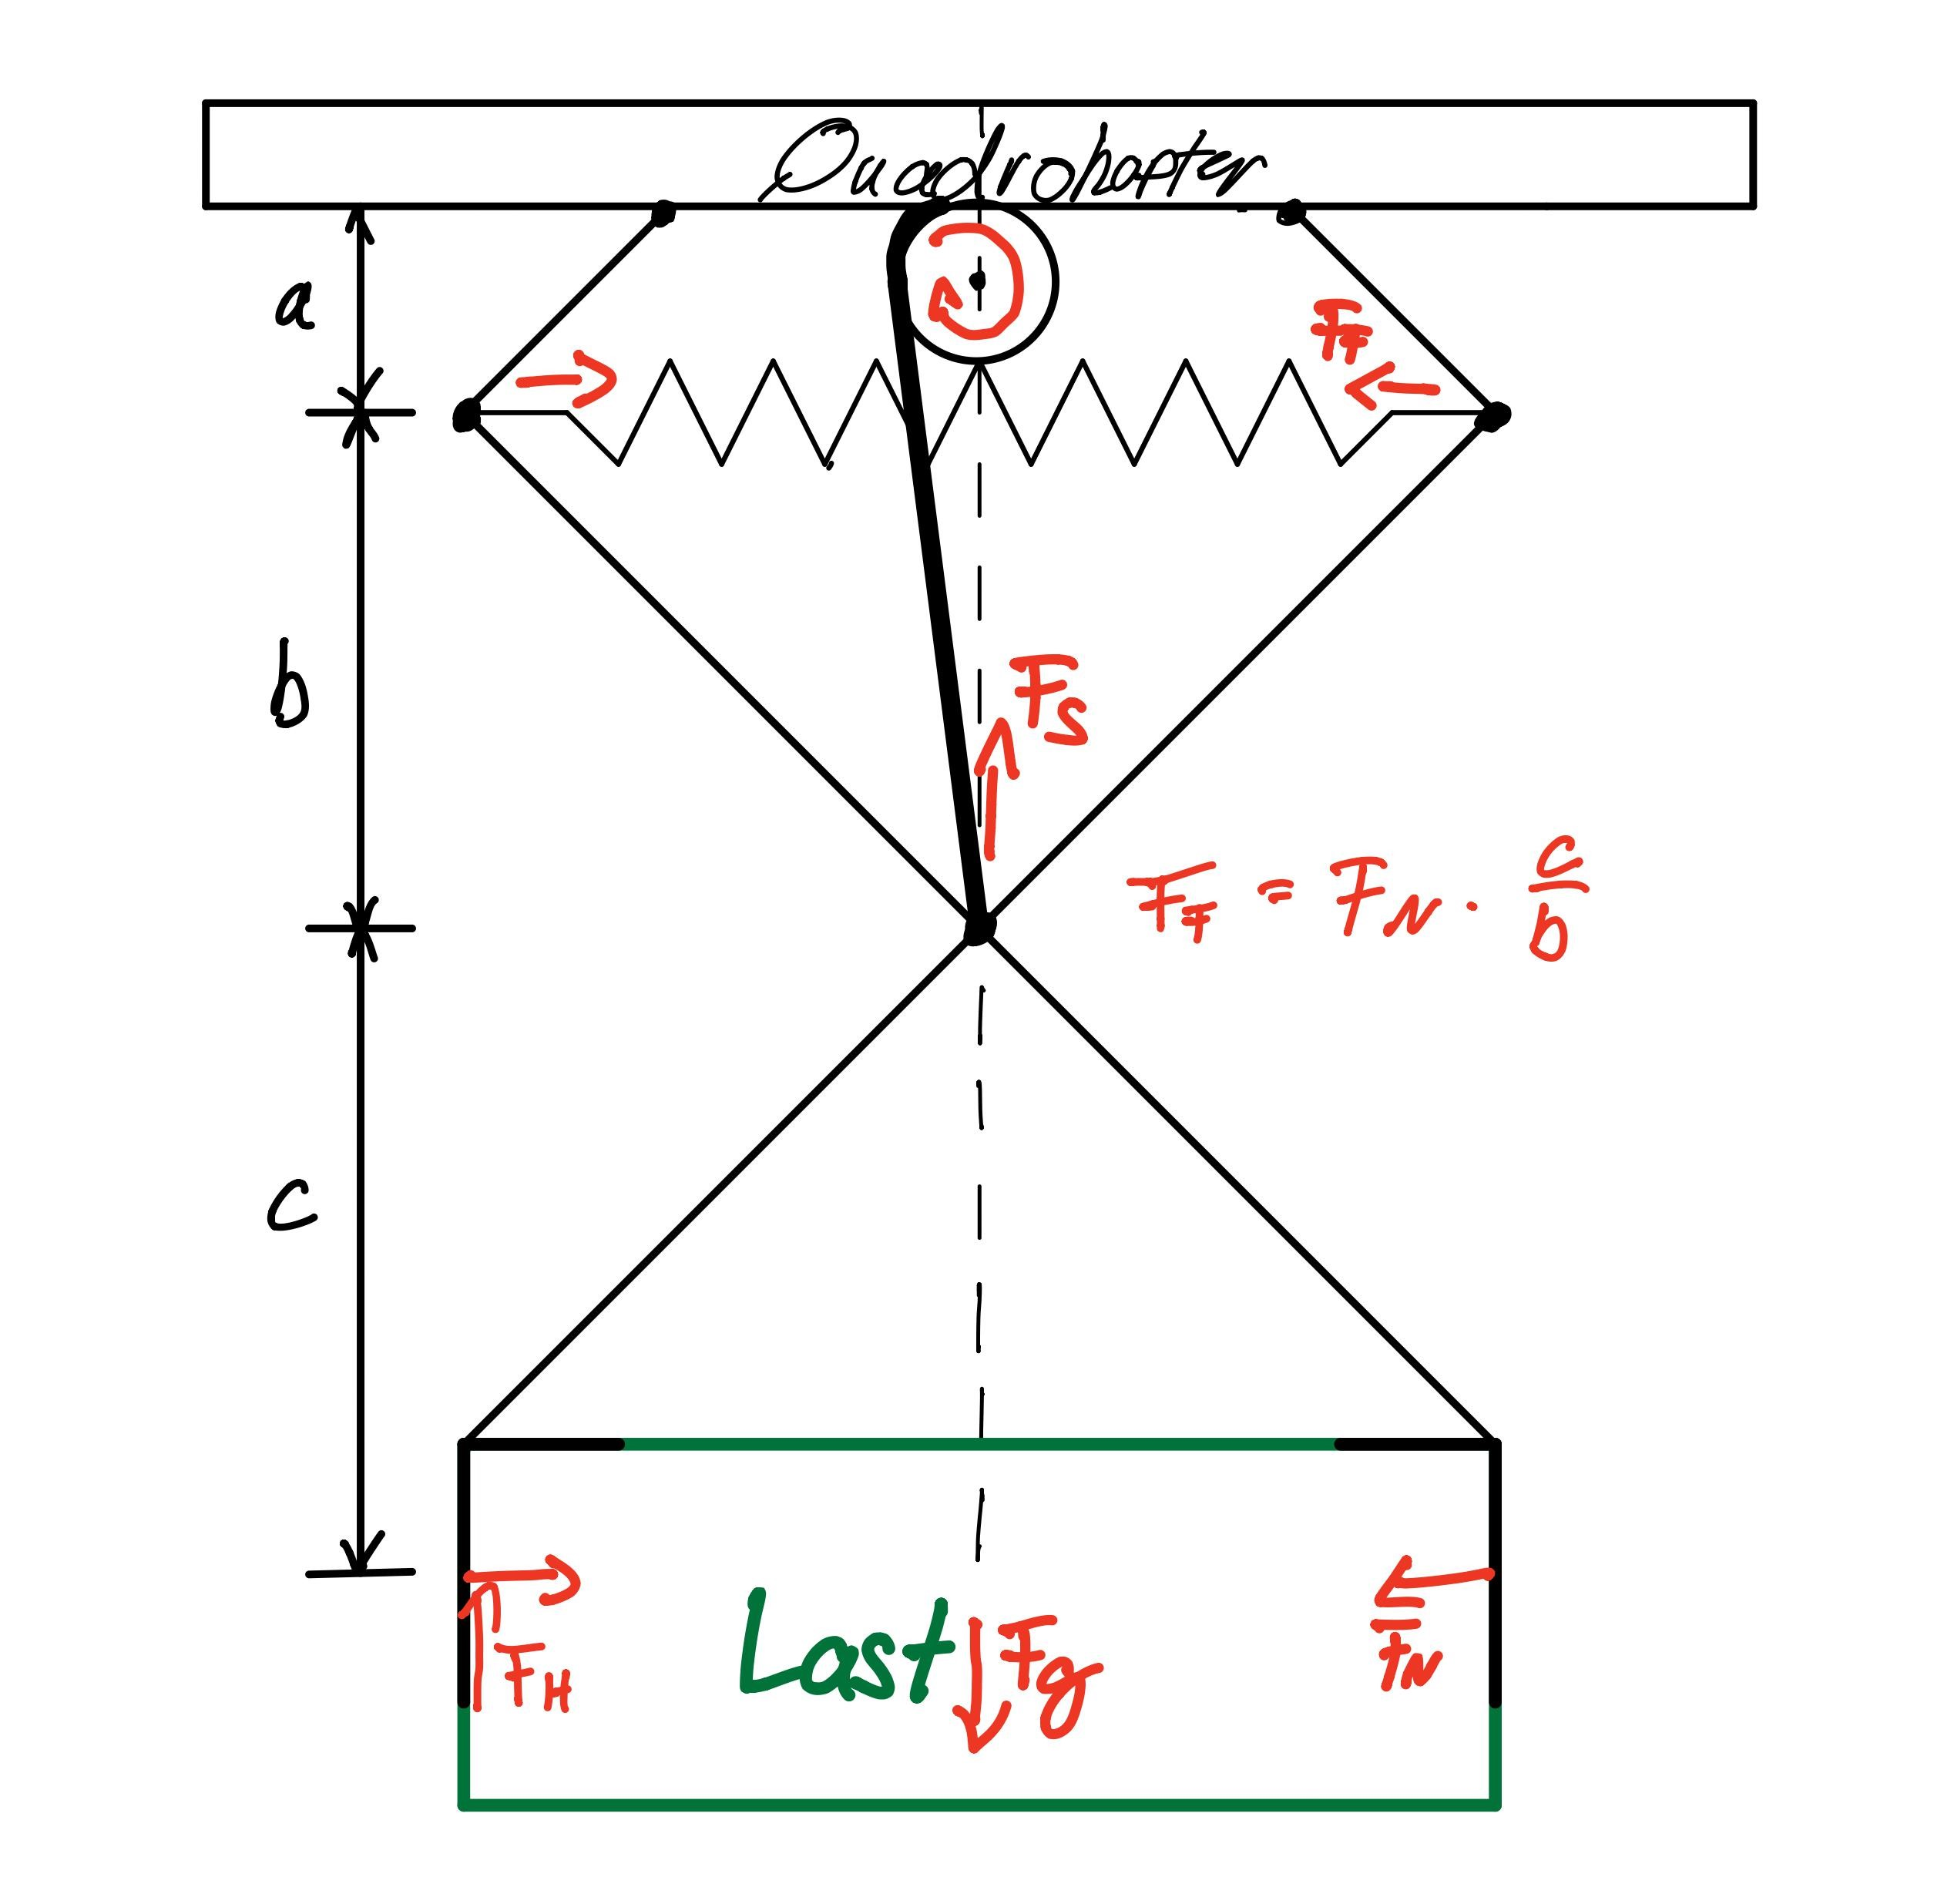
\includegraphics[scale=0.5]{"Grafiken/Skizze1mechanik.png"}
	\caption{Erste Prinzipskizze}
	\label{erste_prinzipskizze}
	\end{center}
\end{figure}

\subsection{2.~Konzept}
Bei der Funktionsweise des zweiten Konzepts aus Abbildung \ref{zweite_prinzipskizze} übernimmt ein elektrischer Hubzylinder die Arbeit. Dieser öffnet und schließt Greifarme und hält diese in Position mit seiner eigenen Steifigkeit.
\\
\\
\begin{figure}[h]
	\begin{center}
	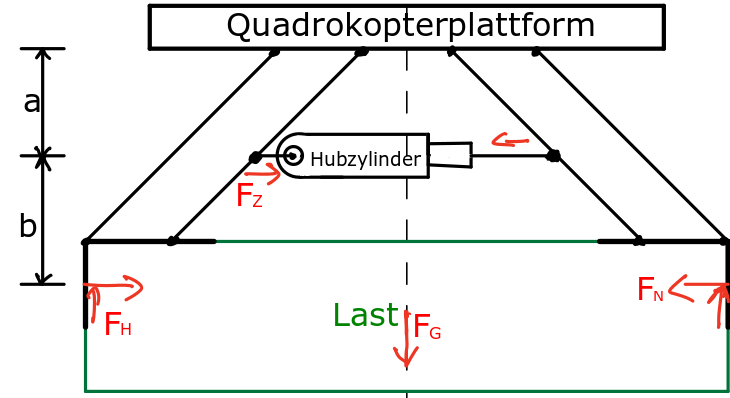
\includegraphics[scale=0.7]{"Grafiken/Skizze2mechanik.png"}
	\caption{Zweite Prinzipskizze}
	\label{zweite_prinzipskizze}
	\end{center}
\end{figure}
\newpage
Auch hinter dem zweiten Konzept steckt ein simples Grundprinzip. Vorteil des Hubzylinders wäre die Steifigkeit, die ohne elektrisches Signal nicht schwindet. Auch ist hier eine parallele Bauweise für mehr Stabilität möglich. Durch den einfach geregelten Hubzylinder, lässt sich die Greifarmbreite beliebig einstellen, wodurch verschieden große Pakete aufgenommen werden können.\\
\\
Jedoch wird trotzdem eine gewisse Präzision beim Ansteuern des Paketes benötigt. Auch ist die Rutschfestigkeit wie beim ersten Konzept nicht gewiss. Zusätzlich wird durch die horizontale Bauweise des Hubzylinders ein großer Bauraum eingenommen.
 
\subsection{3.~Konzept}
Hinter der Funktionsweise des dritten und letzten Konzepts aus Abbildung \ref{dritte_prinzipskizze} verbirgt sich ein Knickgelenk an dessen Ende ein Magnet ist. Dieses Knickgelenk wird mittels zwei Motoren ausgefahren.

\begin{figure}[h]
	\begin{center}
	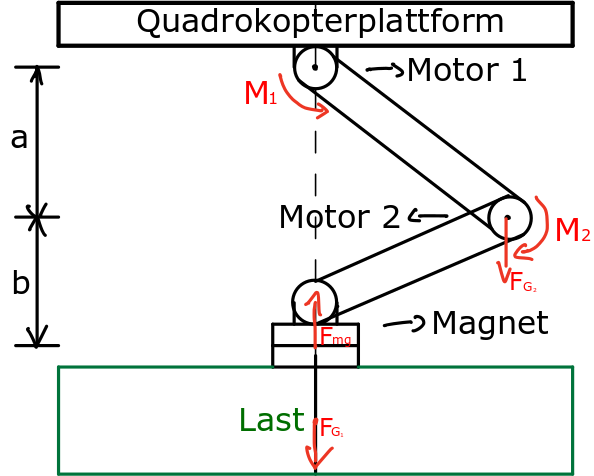
\includegraphics[scale=0.7]{"Grafiken/Skizze3mechanik.png"}
	\caption{Dritte Prinzipskizze}
	\label{dritte_prinzipskizze}
	\end{center}
\end{figure}

Das letzte Konzept ist zwar, durch den zweiten integrierten Motor, etwas komplexer, jedoch entfällt durch den Magneten die Reibungskomponente, was eine erhöhte Zuverlässigkeit bietet. Auch wird dadurch das Ansteuern des Paketes vereinfacht. Durch das Knickgelenk, kann der Schwerpunkt des gesamten Systems sehr gut mittig gehalten werden.\\
\\
Jedoch wird die Gesamtmasse durch den zweiten Motor deutlich erhöht, was auch die maximale Paketmasse niedrig hält. Auch ist die letztendliche Kamera- und Sensorpostion nicht wirklich zentrierbar durch die Lage des Knickgelenks

\subsection{Konzeptauswahl}
Für ein letztendliches Fazit werden Vor- und Nachteile der vorgestellten Konzepte verglichen und abgewogen, um ein finales Konzept auszuwählen.\\
\\
Dabei überzeugt das zweite Konzept aus Abbildung \ref{zweite_prinzipskizze} am meisten, da der Hubzylinder einen stabilisierenden Faktor ins System mit einbringt und sich nur in der Länge verändert, wenn das dafür geeignete Regelgerät das elektrische Signal dafür bekommt. Bei dem ersten Konzept aus Abbildung \ref{erste_prinzipskizze} wäre die konstant benötigte Federkraft zu anfällig auf die anhäufenden Öffnungszyklen. Außerdem sind die simple Bauweise und gleichzeitig stabile Konstruktion des zweiten Konzepts weitere Faktoren, welche für das Konzept sprechen. Gleichzeitig ist ein größerer Spielraum bei der Paketmasse auch ein überzeugender Aspekt, welcher gegen das dritte Konzept aus Abbildung \ref{dritte_prinzipskizze} spricht.\\
\\
Der Hauptfokus liegt demnach im Bauraum und der Länge des elektrischen Hubzylinders, wobei zweiteres als Zukaufteil nicht beliebig variabel ist. Ebenfalls ist die Leistung des Hubzylinders zu beachten, da er bei einem Material wie Plexiglas durchaus in der Lage ist, dieses, bei einem Fehler des Systems, zu zerstören.

\section{Berechnung und Vordimensionierung}
Bei der Berechnung und Vordimensionierung der Greifarmmechanik liegt der Hauptfokus auf dem Bauraum, dem Gewicht des Systems und der letztendlichen benötigten Kraft, welche von dem elektrischen Hubzylinder geleistet werden soll, um das Gewicht fest im Griff zu haben. Ersteres wird durch die Höhe und Lage der Standbeine des Quadrokopters begrenzt. Grobe Messungen ergaben einen Bauraum von  $80\times 80\times130 mm^3$. Dieser lässt sich jedoch durch genaue Formanpassung der Plexiglasteile in die Länge erweitern.

\subsection{Benötigte Normalkraft}
Die letztendlich wichtige Kraft ist die wirkende Hubzylinderkraft, welche in Form der Normalkraft an der Greiffläche wirkt. Letztere lässt sich mittels Reibgesetze berechnen. Da die Greifebene zum tragenden Objekt eben ist, ist die Greifebene zur Horizontalen senkrecht. Die Abbildung \ref{greiferfläche} verdeutlicht die Verteilung der Kräfte.
\begin{figure}[h]
	\begin{center}
	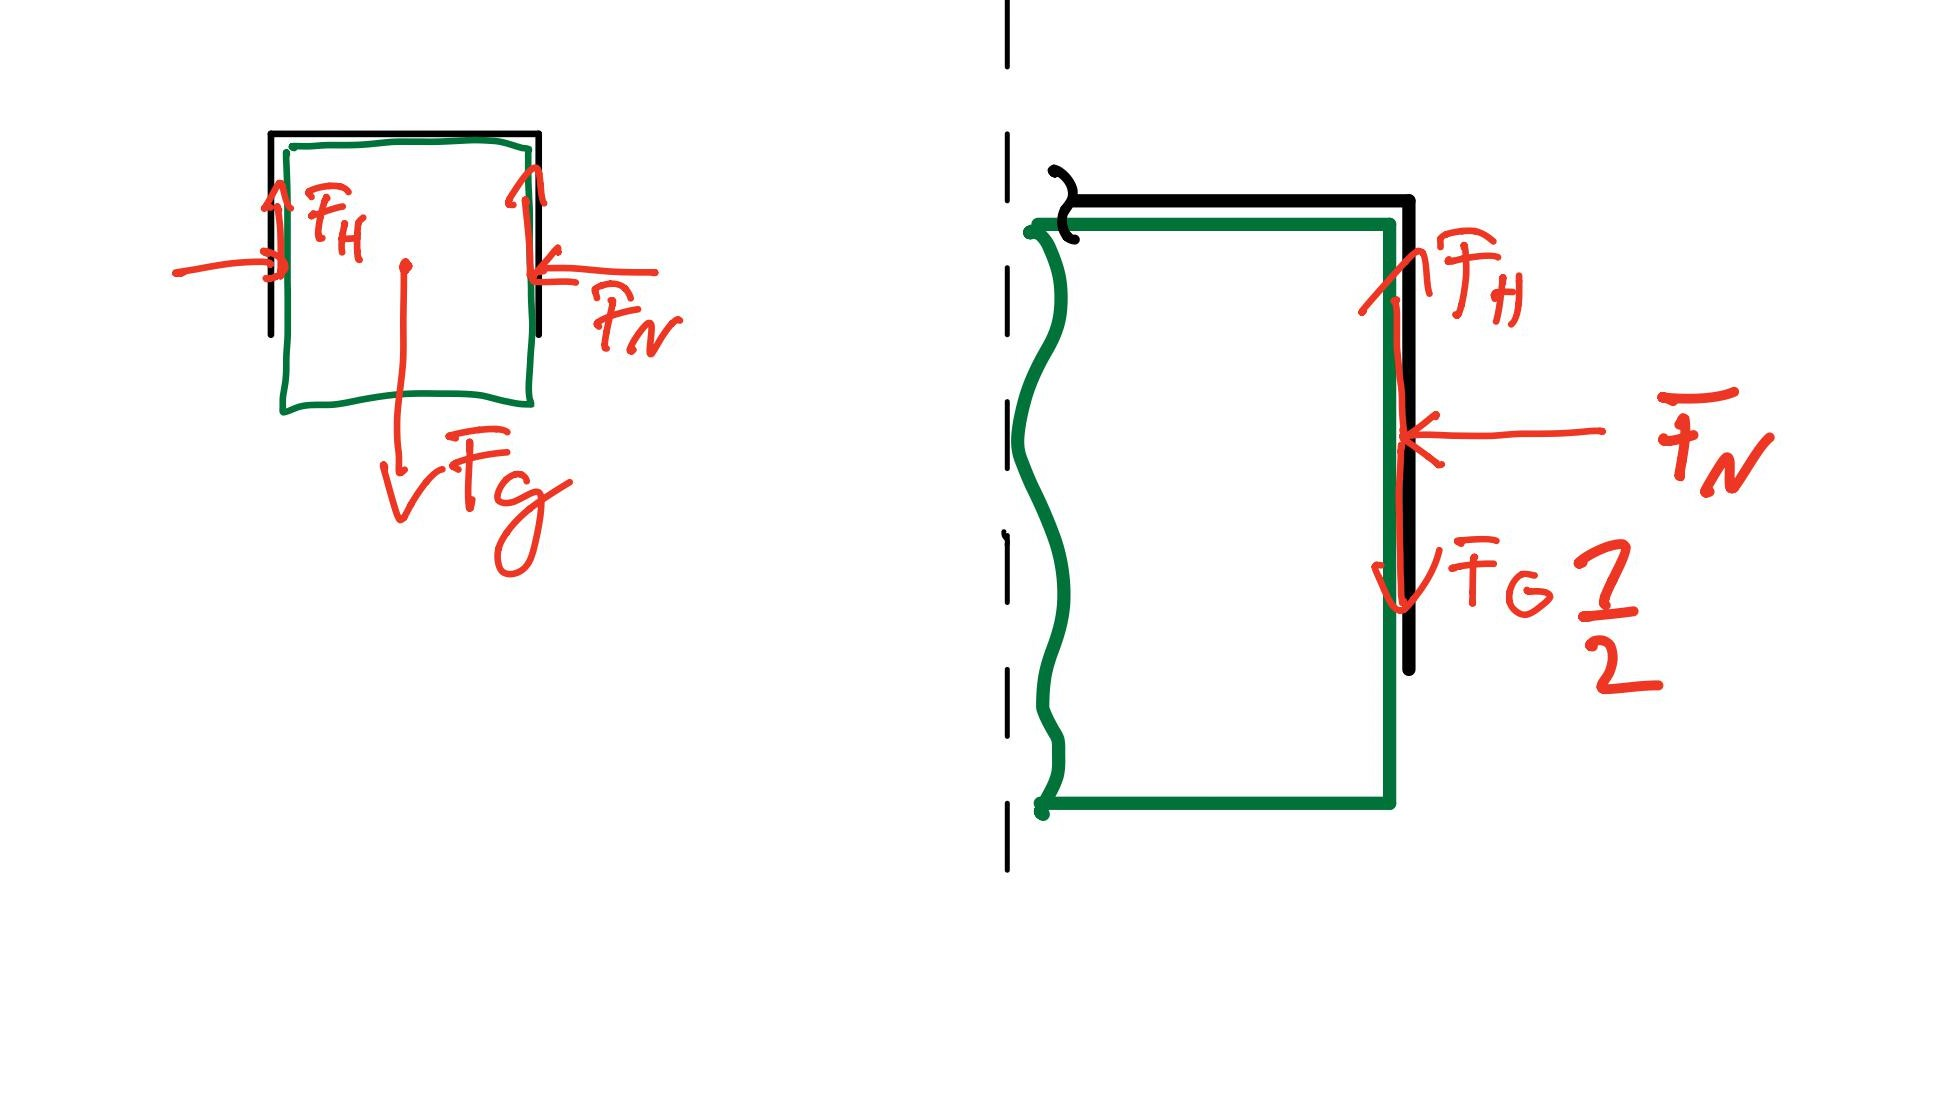
\includegraphics[scale=0.6]{"Grafiken/Greiferflaeche.png"}
	\caption{Kraftverteilung an der Greiferfläche}
	\label{greiferfläche}
	\end{center}
\end{figure}
\newpage
Aus der Abbildung \ref{greiferfläche} ergibt sich, dass die letztendlich benötigte Normalkraft abhängig von der Gewichtskraft und dem Haftreibwert ist. Da sich die Reibwerte zu jeweiligen Gleitebenen verschiedener Materialien nur experimentell erörtern lassen, muss ein Mittelwert genommen werden, welcher nach den ersten Experimenten eventuell zu korrigieren ist. Als Oberflächen werden Gummi und Plexiglas genommen. Nach längerer Recherche setzt sich ein ungefährer Mittelwert von $\mu_H = 0,3$ durch.\footnote[1]{Quelle für Haftreibungszahlen: https://www.chemie.de/lexikon/Haftreibung.html (23.05.2020)}\\
\\
Für die zu ermittelnde Gewichtskraft ist von einem Gewicht von $m=50g$ bis $m=100 g$ für die Last zu schätzen. Um eine gute Fehlertoleranz und damit Sicherheit zu bieten, wird der errechnete Wert mit dem Faktor $S = 1,8$ angepasst.
Mit dem gegebenen Haftreibwert und der Erdbeschleunigung $g = 9,81 \frac{m}{s^2}$ auf die Last, lässt sich nun die nötige Haftkraft in Form der Normalkraft berechnen:

\begin{eqnarray}
\label{erste_berechnung}
\begin{split}
\frac{1}{2}F_G &= F_H  \\
F_G &= mg \\
F_H &= F_N \times \mu_H \\
mg &= 2 F_N \times \mu_H \\
F_N &= \frac{mg}{2\mu_H} \\
	&= \frac{0,1kg\times9,81\times\frac{m}{s^2}}{2\times 0,3} \\
	&= 1,635N \\
F_{Nmin} &= F_N\times S \\
1,635N\times 1,8 &= 2,943N \\
\end{split}
\end{eqnarray}

Aus der Berechnung \eqref{erste_berechnung} ergibt sich also eine ungefähr benötigte Normalkraft von $F_{Nmin} = 3N$.

\subsection{Benötigte Hubzylinderkraft}

Die schlussendlich benötigte Hubzylinderkraft lässt sich über einfache Hebelgesetze mit der Normalkraft schlussfolgern. Anhand der Abbildung \ref{mechanikskizze} und den darauf rotierenden angedeuteten Hebelarmen, erkennt man, dass die maximale Hebellänge in senkrechter Stellung erreicht ist. Die Wahl des Hebelverhältnisses zwischen $a$ und $b$ ist hier entscheidend. Denn Bauraum und Maße der in Frage kommenden Hubzylinder setzen hier starke Grenzen. Für die grobe Vordimensionierung wird das Verhältnis von $a$ zu $b$ auf $1:1$ gesetzt.

\begin{figure}[h]
	\begin{center}
	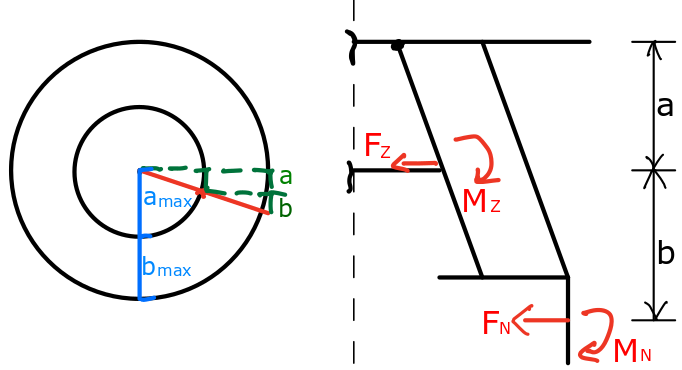
\includegraphics[scale=0.5]{"Grafiken/Mechanikskizze.png"}
	\caption{Kraftverteilung an den Hebelarmen}
	\label{mechanikskizze}
	\end{center}
\end{figure}

\begin{eqnarray}
\label{zweite_berechnung}
\begin{split}
F_N \times(a+b) &= F_Z \times a \\
F_Z &= F_N \times (1 + \frac{b}{a}) \\
 2F_N &= 6N
\end{split}
\end{eqnarray}

\subsection{Auswahl des Hubzylinders}
Mit der in \eqref{zweite_berechnung} berechneten Hubzylinderkraft von $F_Z=6N$ fällt die Wahl des elektrischen Hubzylinders auf den „Titan 30“ von CTI-Modellbau \footnote[1]{Titanzylinder: https://www.cti-modellbau.de/-74-102-110-170-185-328-532.html (23.05.2020)}, welcher mit dem „Thor4HF Titan 1 Regler“, ebenfalls von CTI-Modellbau  \footnote[2]{Titanregler: https://www.cti-modellbau.de/-74-102-110-181-182-191-329-350-543.html (23.05.2020)}, betrieben wird. Durch den begrenzten Bauraum bieten sich nicht viele Alternativen an, da die Firma CTI-Modellbau sich explizit auf den Modellbau konzentriert.
Mit einer erwünschten Öffnungsbreite von jeweils 30 mm pro Seite und einem Faktor von 2, durch die mittige Position des Hubzylinders, lässt sich eine erwünschte Hublänge von 30 mm errechnen.

\section{Vom Modell zu den ersten Bauteilen}
\subsection{Creo Modell}
Mit den ersten vordimensionierten Bauteilen und den ersten festen Maßen von den Zukaufteilen, lässt sich nun ein erstes 3D CAD-Modell bauen. Dabei werden je nach Absprache und Änderungen von Eigenschaften Anpassungen unternommen, um dem finalen Produkt so nah wie möglich zu ähneln. Aus dem CAD Modell aus Abbildung \ref{creo1}, modelliert mit "Creo Parametrics5", lässt sich schon die grobe Gestalt der Greifarmmechanik erkennen. Ausgehend von der Nummerierung in Abbildung \ref{creo1} erkennt man die Bauteile Bodenplatte(1), Hebelarm(2), Führungsschiene(3) und Greifplatte (4). Sie bilden die Grundbausteine des Endprodukts der Greifarmmechanik. Im Zwischenraum von Bodenplatte und Hebelarmen soll später der Hubzylinder(5) Platz finden. Bauteile wie zum Beispiel Verbindungsschrauben oder Abstandshülsen sind außen vor und werden erstmal nicht in der Auflistung berücksichtigt, da diese sich in der Anzahl und der Position noch stark ändern können.
\begin{figure}[h]
	\begin{center}
	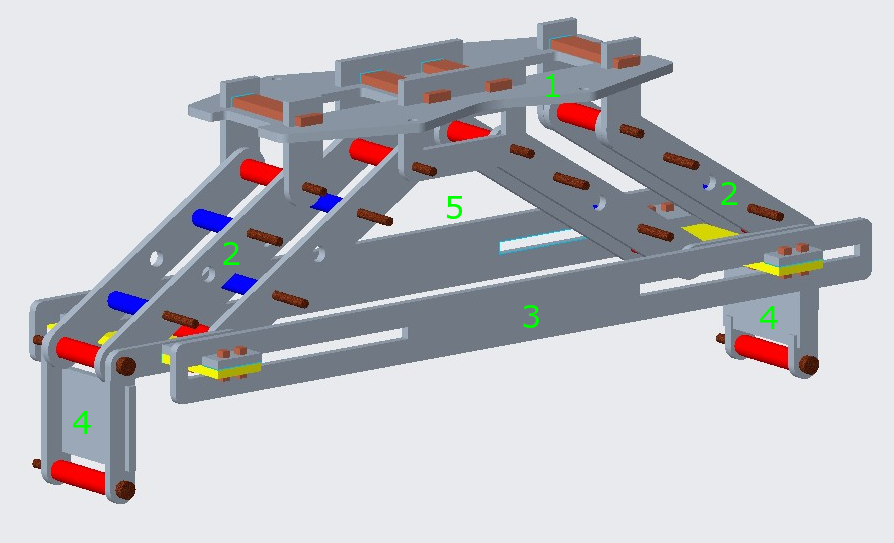
\includegraphics[scale=0.6]{Grafiken/Creo1bearbeitet.png}
	\caption{Erstes CAD-Modelle}
	\label{creo1}
	\end{center}
\end{figure}
\newpage
\subsection{Inkscape}
Die letztendlich fertigen dreidimensionalen CAD-Bauteile können nun mit „Inkscape“, eine Software zur Bearbeitung und Erstellung zweidimensionaler Vektorgrafiken, zu Schnittmustern erzeugt werden. Mithilfe dieser Schnittmuster werden die fertigen Bauteile zweidimensional aus den Plexiglasplatten mit konstanter Wandstärke von der Laserschneidemaschine ausgeschnitten. Dementsprechend ist bei der Konstruktion der Bauteile zu beachten, dass diese zweidimensional als Schnittmuster abgebildet werden können.

\begin{figure}[h]
\begin{center}
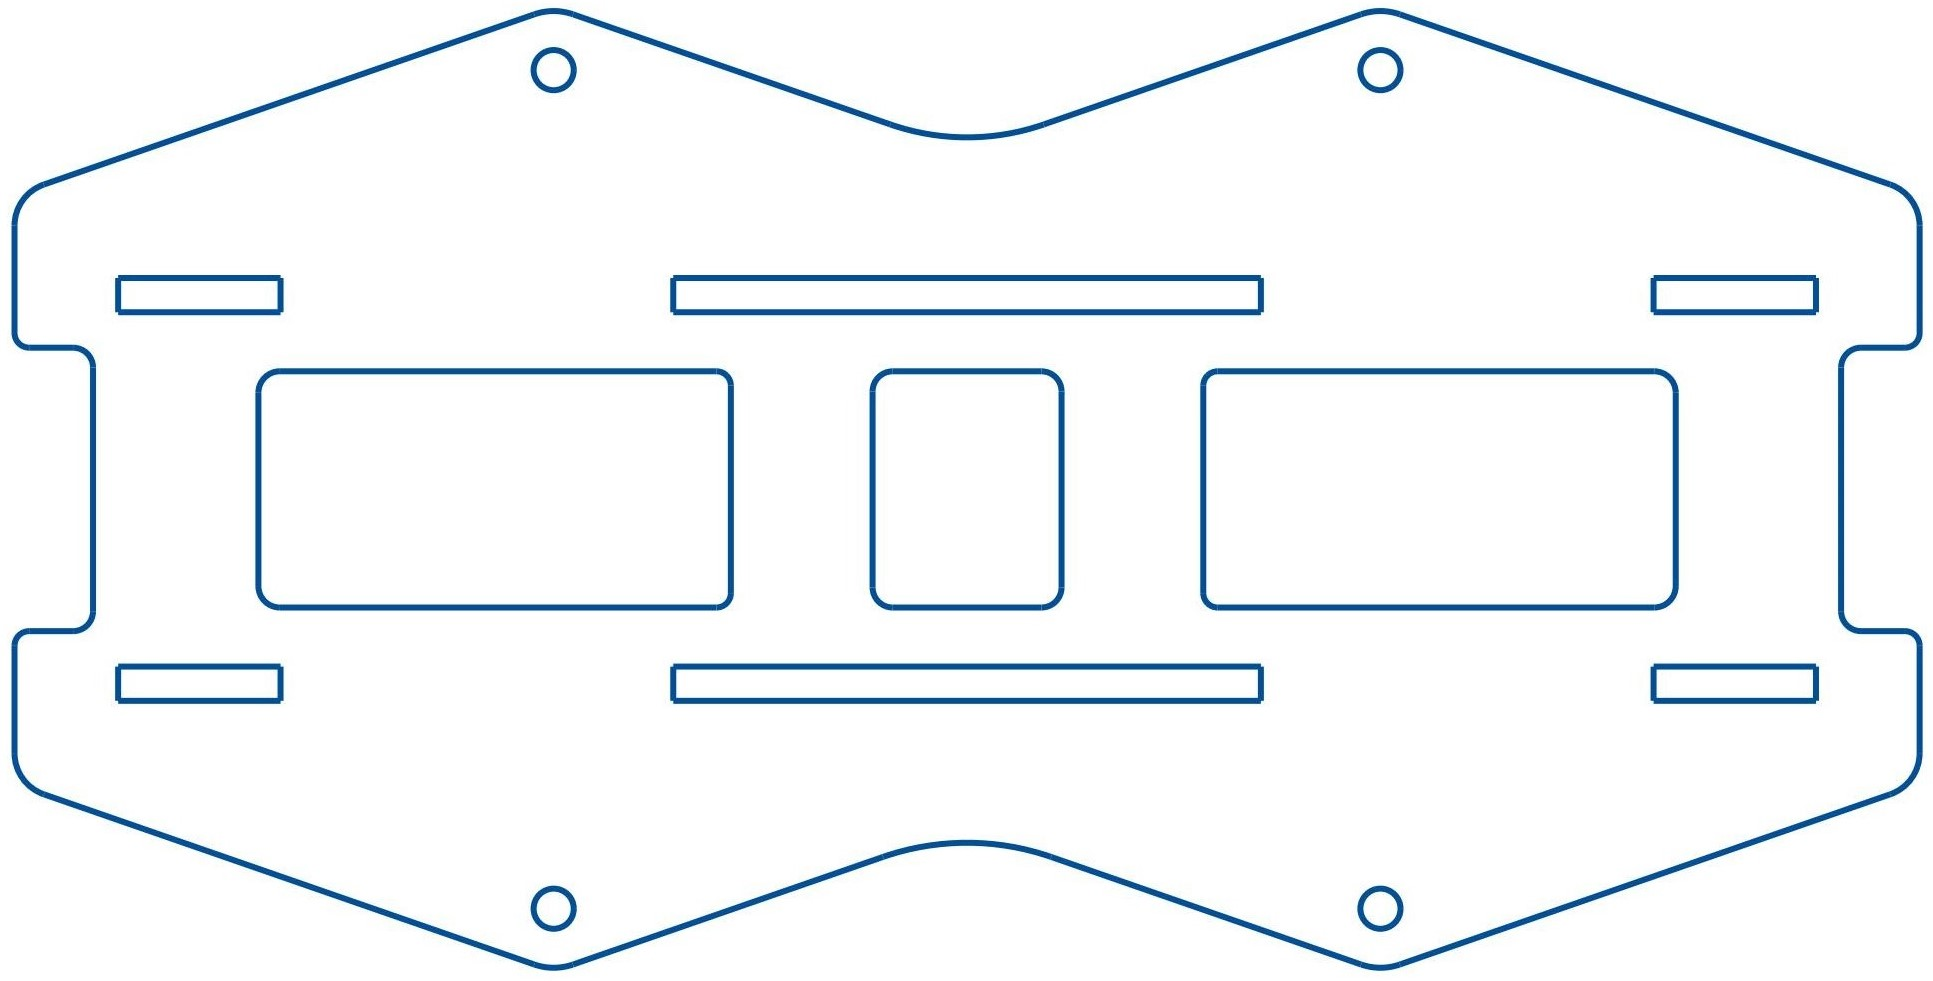
\includegraphics[scale=0.5]{Grafiken/Inkscapebodenplatte.jpg}
\caption{Inkscapeschnittmuster der neuen Bodenplatte}
\label{inkscape1}
\end{center}
\end{figure}

\subsection{Erste Ergebnisse}
Die ausgeschnittenen Bauteile werden zur Probe vormontiert, um mögliche Problemstellen ausfindig zu machen. Die Abbildungen \ref{hebelarme} und \ref{vormontage} zeigen erste Montageversuche.

\begin{figure}[h]
\begin{center}
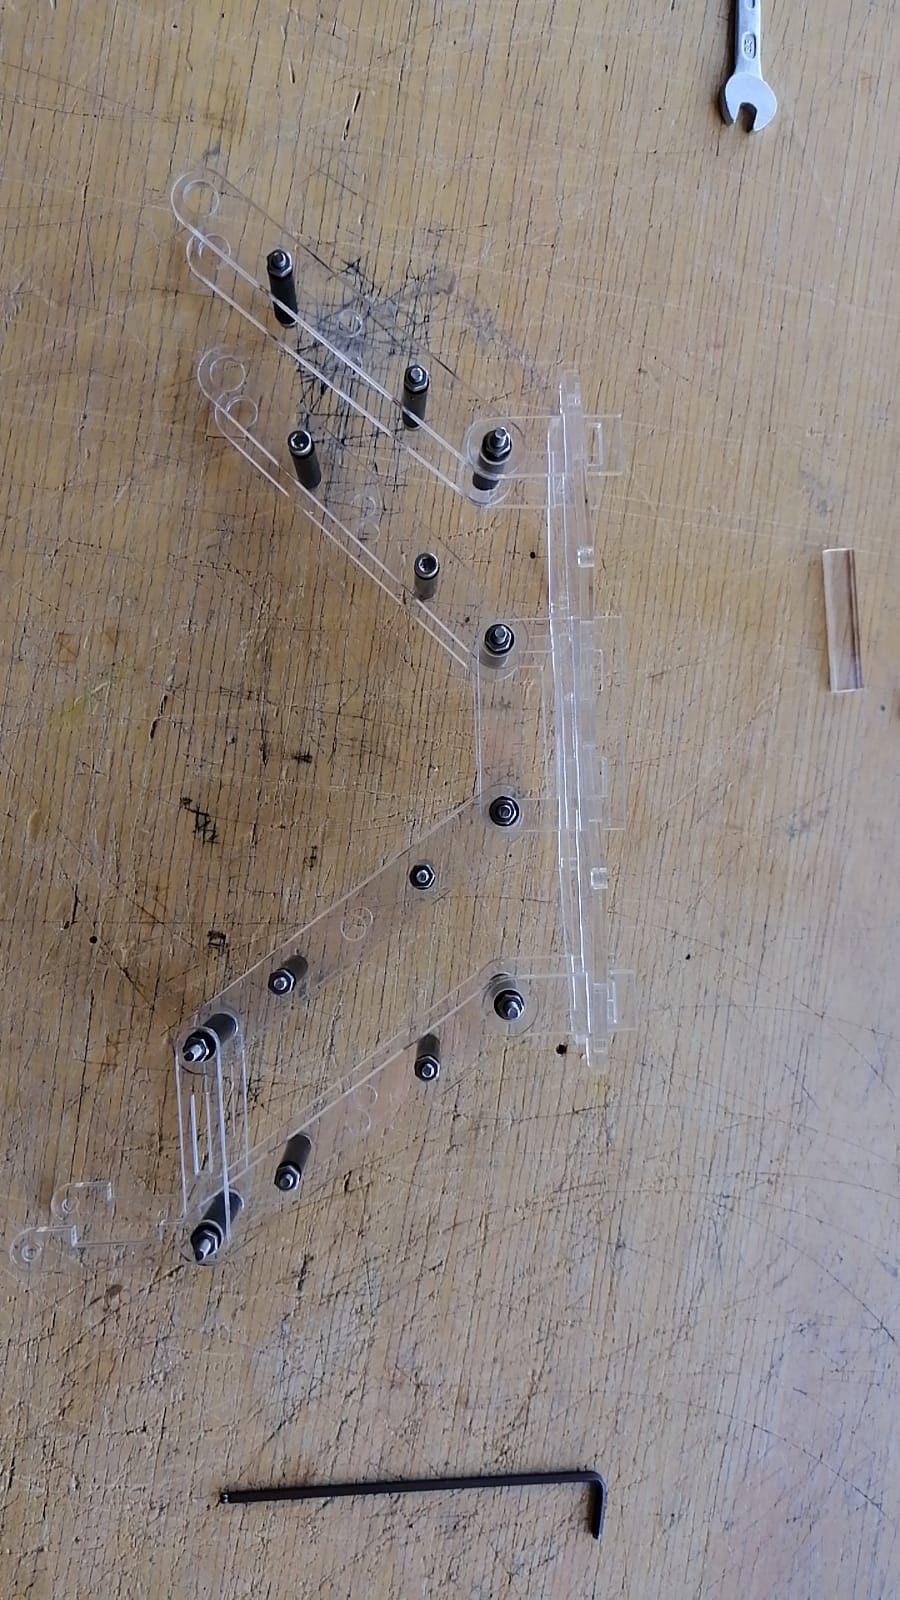
\includegraphics[angle=90,scale=0.3]{Grafiken/Fotohebelarme.jpg}
\caption{Zusammengebaute Hebelarme}
\label{hebelarme}
\end{center}
\end{figure}

\begin{figure}[h]
\begin{center}
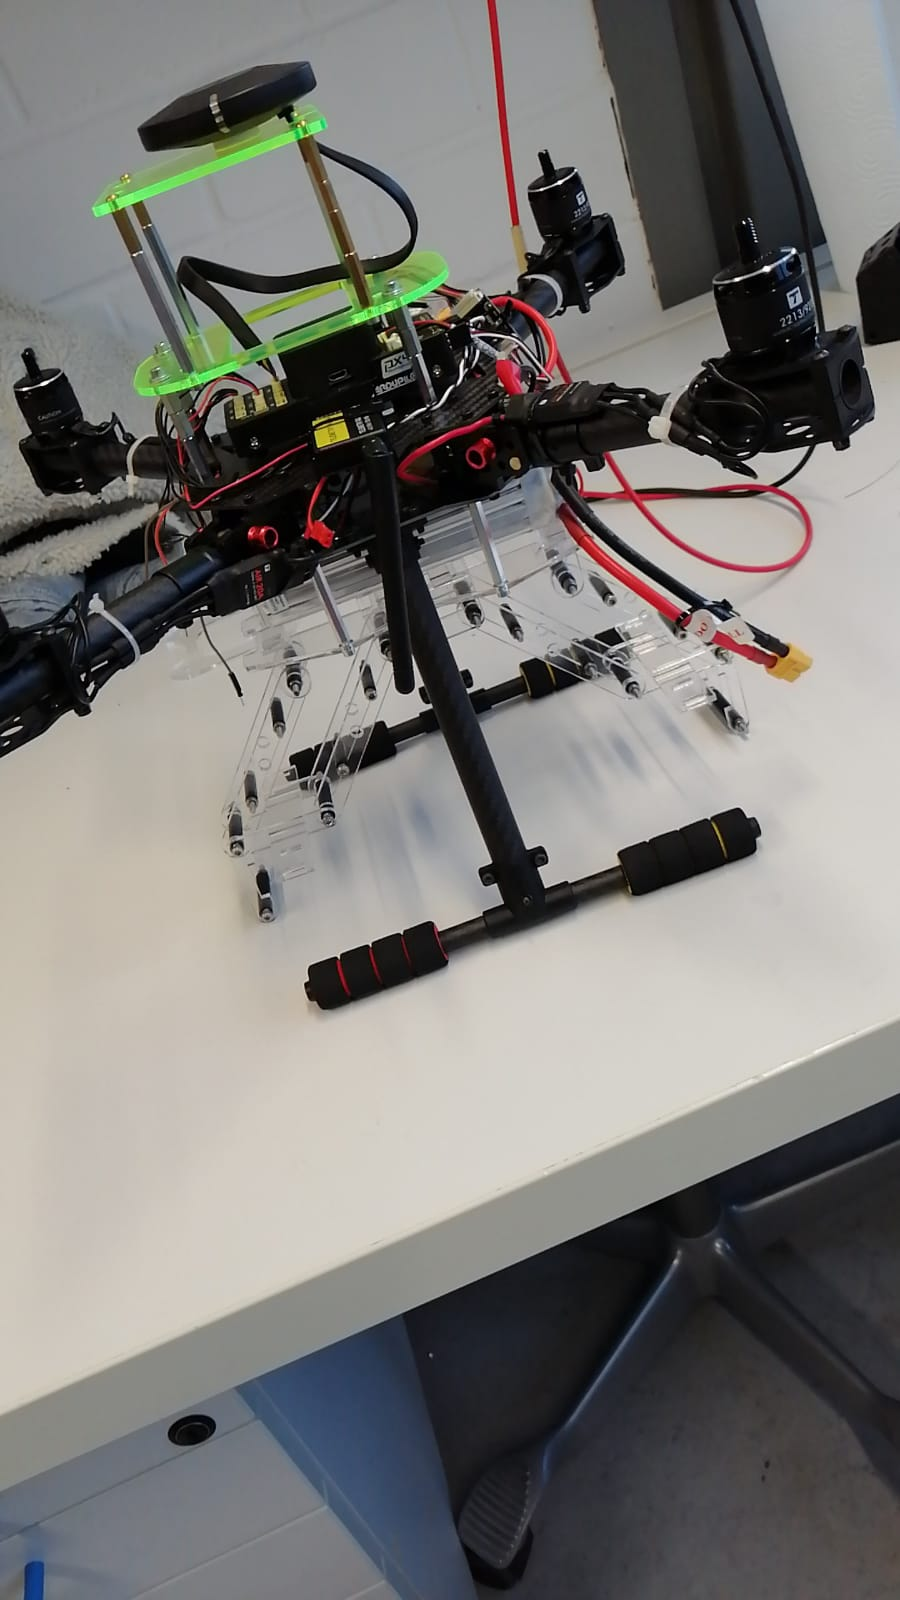
\includegraphics[scale=0.4]{Grafiken/Fotoquadrokopter.jpg}
\caption{Vormontage der Greifarmmechanik am Quadrokopter}
\label{vormontage}
\end{center}
\end{figure}
Um die aus den Berechnungen gewünschte Reibung zu erlangen wird auf den Flächen der Greiferplatten (Nummer 4 in Abbildung \ref{creo1}) noch eine Gummischicht draufgeklebt.
Nach der letztendlich fertigen Konstruktion muss für die Sensoren noch eine Befestigung hinzugefügt werden. Diese ist aber letztendlich stark vom eingenommenen Volumen des Greifsystems im Bauraum abhängig, da sie bestenfalls zentriert liegt und wird erst nach den ersten Testläufen beigefügt

\section{Problematiken und Lösungen}
Bei den ersten Testläufen ist vermehrt aufgefallen, dass die Wandstärken mit dem CAD Modell schlecht einschätzbar sind und demnach lange und dünne Bauteile wie zum Beispiel die Führungsschienen (Nummer 3 in Abbildung \ref{creo1}) so umkonstruiert werden müssen, damit die gewollte Steifigkeit von dem benutzten Plexiglas trotzdem noch erhalten bleibt.\\
\\
Gleichzeitig muss auf die Anziehkraft der Schrauben geachtet werden, da bei zu hohen Kräften das Plexiglas durchbrechen könnte oder auch zu hohen Reibungskräften unterliegen würde, welche das System zu sehr unkontrolliert beeinflussen würde. Demnach sind alle Schrauben nicht komplett versteift eingeschraubt, was gleichzeitig zur Folge hat, dass Steifigkeit und Stabilität des Systems in gewissen Maßen drunter leiden. \\
\\
Auch funktioniert die Führungsschiene nicht so wie angedacht, da zu hohe Reibungskräfte zwischen den einzelnen Plexiglasflächen entstehen. Ein kurzer Umbau lässt nun die Führungsschiene das System, über die schon angebrachten Bolzen, an den Greifern führen. Auch diese Lösung ist nicht perfekt, denn wenn die Querkräfte zu hoch werden, verbiegt sich das Plexiglas und erfüllt demnach nicht mehr seine Funktion einwandfrei. Auch das ist mit einer erhöhten Wandstärke auf Kosten höheren Gewichts teilweise besser geworden. Da aber auch hier die Reibung zwischen Führungsbolzen und Plexiglas nicht komplett zu verhindern ist, lässt sich das Problem nicht ganz lösen.\\
\\
Ein weiteres Problem ist der Öffnungswinkel des Systems. Denn um 60 mm gewollten Öffnungsspalt zu erreichen, müssten die Hebel weiter voneinander entfernt liegen, was das Volumen des Greifarms noch größer machen würde. Denn die Länge des Hubzylinders ist nicht stark variabel, weshalb der Bauraum zur Mitte hin begrenzt ist. Der momentane Öffnungsspalt von 45 mm sollte demnach erstmal beibehalten werden, da Verbesserungen größere Maßnahmen erfordern würden.
\section{Fazit zur Mechanik}

Bei der letztendlichen Fertigstellung der Mechanik zeigt sich die Komplexität darin die Balance zwischen Leichtbau, Stabilität und Steifigkeit beizubehalten, ohne dabei die Funktion des Greifarms einzuschränken und das mit einfachsten Mitteln. Der Verzicht auf einen Elektromagneten für die Greiffunktion führt zu einem großen eingenommenen Bauraum und viel Zusatzgewicht, da die Konstruktion der Greifarme für die anliegenden Kräfte eine gewisse Stabilität brauchen. In realitätsnahen Szenarien werden Faktoren wie zuverlässige Stabilität und möglichst lange Akkulaufzeiten jedoch benötigt. Dies stellt sich als eine zukünftige Hürde für andere Projekte dieser Art heraus. Die Grundfunktion an sich wird jedoch erfüllt.\\
\\
Das Bauen ohne zuverlässige Lagerung erwies sich auch nicht als einfach und kostete dem System weitere Stabilität. Auch der enorme Bauraum, generiert durch den Hubzylinder, setzt dem System starke Grenzen und führt zu einem erhöhten Gewicht.

	\chapter{Sesorik, Aktorik und andere Hardware}
	\chapter{Softwareimplementierung}
\section{Softwareanforderung}
Ein weiterer Teil des Projektes ist die Softwareimplementierung. Die Aufgabe dieser erstreckt sich von der Bildverarbeitung über den Objekterkennungsprozess bis hin zu der Regelung und Steuerung der Drohne. Dabei muss sie verschiedensten Kriterien genügen.\\
\\
Da sie Signale von einem Externen Bauteilen wie dem PX4 oder dem Abstandssensor über das Interface ROS (siehe Kapitel \ref{gesamtintegration}) kann es zu Datenverlust kommen. Bedingt durch die unterschiedlichen Taktrate der Prozessoren. Deshalb muss auch bei gelegentlich fehlenden Datenpaketen der Rest verarbeitet und die Drohne auf Grundlage dieser geregelt werden.\\
\\
Der PX4-Controller schreibt eine Datenrate von 20 Hz vor. Also muss in dieser Datenrate die Sollposition der Drohne geschickt werden. Fallen diese aus, so geht die Drohne in den Offboard-Modus und steigt auf 10 m Höhe, um dann automatisch zur Startposition zurückzukehren. Dies wäre bei einer Raumhöhe von 2,5 m fatal. Leider kann man diese „Schutzfunktion“ nicht abschalten da sie fest im Betriebssystem des PX4-Controllers verankert ist. Demzufolge darf das Signal der Position nie ausbleiben.\\
\\
Um dies zu erreichen, darf sich die Regeleinheit der Drohne nie aufhängen. Alle Schleifen müssen deshalb ein zeitliches Abbruchsignal haben, um eine Auslastung des Arbeitsspeichers zu verhindern. Aufgrund des Gewichtes muss ein leichter Controller gewählt werden(siehe Hardware Komponenten). Da wir aufgrund der Software Inkompatibilität des Pi-4 mit dem PX4-Controller einen Pi-3 gewählt haben steht ein maximaler Arbeitsspeicher von 1 Gb zur Verfügung. Dabei hat er 2 Kerne und kann somit effektiv 2 Aufgaben gleichzeitig ausführen. Die Software muss also sehr ressourcensparend geschrieben sein.\\
\\
Aufgrund der Struktur von ROS empfiehlt es sich, einen Event basierten Programmablauf zu schreiben. Dabei löst ein Event, also eine Aktion die stattfindet, einen Programmablauf aus. In diesem Fall sind die Events eingehende Datenpakete für die entsprechende Node (Siehe Programmstruktur). Diese werden verarbeitet. Dadurch kann sichergestellt werden, dass jedes Datenpaket verarbeitet wird, unabhängig in welchem Abstand es ankommt. Durch diese Warte-Bedien-Struktur wird eine maximale Effizienz erreicht, da das Programm keine Schritte doppelt auf nicht aktualisierte Werte anwendet und so Prozessorzeit spart.
\section{Python als Programmiersprache}
Wie es häufig in der Entwicklung der Fall ist, stehen auch hier für die Implementierung
der Software auf dem RPi verschiedene Plattformen, Frameworks und
Programmiersprachen zu Verfügung. Bei der Wahl der Programmiersprache ist zu beachten das sie möglichst einfach und bereits relativ alt ist. Der Vorteil von alten Programmiersprachen ist, dass es eine umfangreiche Beispielsammlung gibt. Dadurch kann man sich leicht an bereits vorhandenem Code orientieren.
Anforderungs-bedingt muss die Programmiersprache möglichst ressourcenschonend sein.
Dadurch fallen alle grafischen Programmiersprachen wie Matlab, Simulink, Labview etc. heraus. Diese haben aufgrund ihres unstrukturierten Programmablaufs, eine eher schlechte Laufzeit.\\ 

Eine der am weitesten verbreiteten Programmiersprachen ist Java. Der Vorteil von Java ist, dass es plattformübergreifend funktioniert. Leider verwendet Java dafür eine Virtuelle Java Maschine. Also ein Betriebssystem, dass noch mal über dem Betriebssystem liegt. Dies verringert die Laufzeit von Java enorm. Ein weiteres Problem liegt darin, dass Schnittstellen immer plattformabhängig sind(USB, D-Sub, Ethernet etc.). Dadurch werden sie durch Java nur schlecht unterstützt. Aus diesen Gründen konnte Java ebenfalls nicht gewählt werden.\\

Eine weitere Alternative ist eine C-Programmiersprache(C++, C etc.). Diese haben den großen Vorteil, dass sie echtzeitfähig sind. Sie können also unter Umständen garantieren, dass das Ergebnis des Algorithmus nach einer bestimmten Zeit feststeht. Dies ist für eine Drohnensteuerung sehr geeignet, da man garantieren sollte, dass sie Drohne in einem bestimmten Zeitintervall überwacht wird. Außerdem sind C-Sprachen sehr Hardware nah geschrieben, wodurch die Laufzeit sehr gut ist. Allerdings wird die Hought-Transformation der Bibliothek Open-CV genutzt. Diese Bibliothek ist allerdings nicht echtzeitfähig, wodurch der große Vorteil von C verloren geht. Des Weiteren ist es sehr schwer/mühselig Open-CV in C zu implementieren.\\

Außerdem ist Python eine Alternative. Python ist leider nicht echtzeitfähig. Jedoch ist es sehr benutzerfreundlich, hinsichtlich des Importierens von Bibliotheken. Es ist nicht so hardwarenah wie C, allerdings immer noch deutlich näher als Java oder Labview. Außerdem gibt es zahlreiche Beispiele für Python und das Ansteuern von Schnittstellen geht problemlos. Aus all diesen Gründen ist die Wahl auf Python gefallen.

\section{Vergleich Monolithische Single Application und Service Oriented Architecture}
\subsection{Monolithische Single Application}
Bei der Softwarearchitektur wurde sich zunächst an einer normalen objektorientierten Struktur bedient: Es gibt eine main-Datei, welche vergleichsweise
klein ist und nur die grobe Struktur bzw. den Gesamtablauf darstellt. Diese ruft dann weitere Softwaremodule auf, die die Unteraufgaben, wie beispielsweise das Empfangen und Verarbeiten von Bilddaten, implementiert. Ein Problem, das hier recht schnell auftritt ist, dass theoretisch zwei Prozesse gleichzeitig ablaufen müssen. Wenn ein Motormodul beispielsweise gerade darauf wartet, dass die Sollposition erreicht wurde, müsste in einem Programmierstrang, in dem ein Befehl nach dem anderen ausgeführt wird, das Kameramodul mit der Verarbeitung des Bildes auf das Motormodul warten, obwohl das Motormodul gerade gar nichts tut, außer auf den
Motor in der echten Welt zu warten, bis er die gewünschte Position hat. Da das Kameramodul aber an das Motormodul eventuell kommunizieren muss, dass das
Paket gar nicht mehr an der richtigen Stelle ist, weil der Quadrokopter aufgrund äußerer Umstände nicht ganz stillsteht, müssen beide Module gleichzeitig arbeiten und
miteinander kommunizieren können. \\

In der traditionellen Softwareentwicklung gibt es dafür sogenannte Threads. Diese sind separate Ausführungsstränge, die quasi gleichzeitig ausgeführt werden und sich dann beispielsweise ein Datenobjekt im Speicher teilen und über dieses miteinander kommunizieren können. Das entspricht dann einer Dreischicht-Architektur (siehe Abb. \ref{fig:Dreischichtarchitektur}).

Wichtig bei dieser Art der Architektur ist, dass jede Schicht nur auf die nächst untere zugreifen darf, um einen reibungslosen Ablauf garantieren zu können. In diesem Fall greifen nun die Threads $T_1$, $T_2$ ... $T_n$ nicht direkt auf den Speicher zu, sondern müssen den Weg über die Datenzugriffsschicht gehen. Diese stellt unter anderem mittels Semaphoren sicher, dass immer nur ein Thread auf die entsprechende Ressource zugreifen kann. Damit wird verhindert, dass beispielsweise $T_1$ schreiben und $T_2$ gleichzeitig lesen möchte. Dies würde zu einem Speicherkonflikt führen und das Programm wird abstürzen. \cite{riedel2019itarch}

\begin{figure}[h]
	\centering
	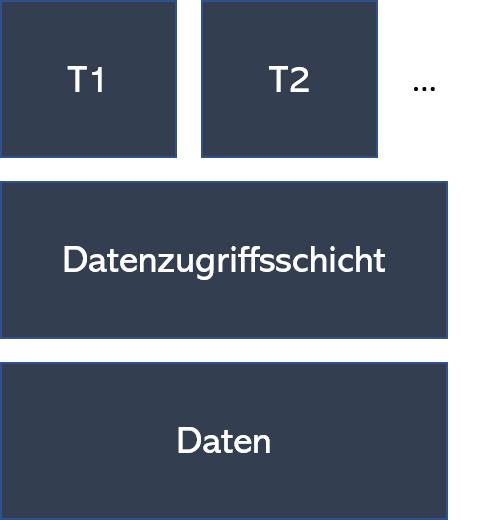
\includegraphics[scale=0.5]{"Grafiken/dreischichtarchitektur.png"}
	\caption{Dreischichtarchitektur}
	\label{fig:Dreischichtarchitektur}
\end{figure}



\subsection{Service Oriented Architecture}
Bis zu einem gewissen Grad war es möglich die geforderten Funktionalitäten mit Multithreading zu implementieren. Allerdings wurde es im Laufe der Entwicklung immer komplizierter, da Bilddaten beispielsweise von zwei Ressourcen abhängen, die nicht immer verfügbar sind: zum einen der Speicherplatz im Datenobjekt, das andere Threads lesen und damit belegen wollen und zum anderen von der Kamera selbst, die natürlich auch nicht willkürlich Bilddaten liefert. Das zu synchronisieren ist zwar theoretisch möglich, praktisch aber mit einer Menge schwer wartbarem Code verbunden, der das Problem unnötig kompliziert löst.
\subsection{Robot Operating System}
Deshalb basiert die endgültige Software auf ROS, das genau diese Probleme adressiert. ROS steht dabei für Robot Operating System und ist ein Framework, das auf dem Publisher-Subscriber-Modell (P/S-Modell) basiert. Die Idee ist dabei, dass es verschiedene Themen (Topics) gibt, in die verschiedene dezentrale Skripte, die gleichzeitig laufen, Informationen zu einzelnen Themen veröffentlichen oder abonnieren können. So gibt es beispielsweise ein Kameraskript, das das Bild und die erkannte Position des Pakets veröffentlicht und ein Motorskript abonniert die Paketposition und kann daraus dann weitere Schlüsse ziehen. Ein anderes Skript könnte dann auf einem anderen Rechner (z.B. Laptop) im gleichen (WLAN-) Netzwerk das Kamerabild abbonnieren und mit sehr wenig Programmieraufwand anzeigen. Das elegante dabei ist, dass sämtliche vorher beschriebene Multithreading-Probleme dabei vom sogenannten ROS-Core, der zentrale Schaltstelle des ROS, übernommen werden und damit die einzelnen (selbstgeschriebenen) Skripte sehr entschlackt werden. Das macht es deutlich einfacher diese zu debuggen. ROS ist zudem sehr gut dokumentiert und für viele Probleme gibt es bereits vorgefertigte Skripte, die Dank des einfachen P/S-Modells auch einfach anzubinden sind.
\subsection{ROS als Beispiel einer Service Oriented Architecture (SOA) / Microservices}
Die Architektur hinter ROS ist dabei keine neue Erfindungen, sondern basiert im Gegensatz zum Ansatz der Schichtenarchitektur auf dem Prinzip der serviceorientierten Architektur (SOA). 
\begin{figure}[h]
	\centering
	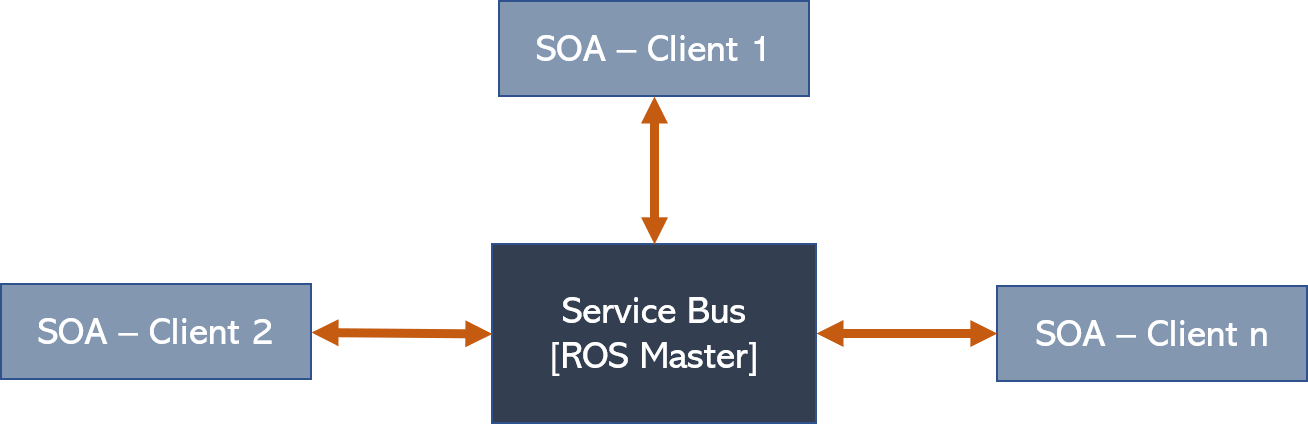
\includegraphics[scale=0.5]{"Grafiken/soa.png"}
	\caption{Service Oriented Architecture}
	\label{fig:meine-grafik}
\end{figure}
Bei der SOA spielt der (Enterprise) Service Bus eine zentrale Rolle. Er ist das Bindeglied zwischen allen anderen Knotenpunkten im Netzwerk und stellt sicher, dass die Kommunikation funktioniert. Bei ROS ist das der ROS-Master, der über den Befehl 
\begin{lstlisting}[language=bash]
$ roscore
\end{lstlisting}
gestartet werden kann. Über ihn kommunizieren die Knoten miteinander, wobei jeder Knoten eine logisch abgeschlossene Aufgabe übernimmt und von außen über eine API angesprochen werden kann. Im Fall des Quadrokopters existiert nun beispielsweise ein Knoten, der das Kamerabild publiziert, einer, der das Bild verarbeitet und einer, der die Steuerung auf Basis der Bilddaten durchführt. Durch diese Modularität gibt es einige Vorteile. So ist es damit sehr leicht einen Knoten auszutauschen, zu erweitern oder neue Knoten hinzuzufügen. Zudem ist das System deutlich stabiler als eine monolithische Lösung, da bei einem fehlerhaften Knoten nur die Knoten ausfallen, die von diesem Ausfall logisch betroffen sind. Alle unabhängigen Knoten werden weiterhin funktionieren. Bei einer monolithischen Lösung führt ein Modulausfall zum Ausfall des Gesamtsystems. 

Aber einer gewissen Granularität spricht man von Microservices. Diese folgen der Strategie 
``Erledige nur eine Aufgabe und erledige sie gut'' %ToDo:\cite{riedel:it-arch}
Bei ``normalen'' SOAs sind die Knoten tendenziell groß und implementieren viele Funktionalitäten auf einmal. Microservices hingegen sind sehr klein und erledigen nur eine bestimmte Aufgabe. In der finalen Gesamtarchitektur kommen Knoten zum Einsatz, die sowohl den normalen SOAs als auch den Microservices zugewiesen werden können.

\section{Finale Gesamtarchitektur}
In der finalen Gesamtarchitektur (siehe Abb. \ref{fig:gesamtarch}) gibt es insgesamt drei ROS Instanzen: Die erste läuft auf dem Quadrokopter selber und dient als Schnittstelle zur Firmware des Quadrokopters. Der dazugehörige Knoten heißt Mavros, welcher mit MAVLink (Micro Air Vehicle Link) kommuniziert, das die gesamte tatsächliche Steuerung des Quadrokopters übernimmt. Dabei hat der ROS-Core jedoch keine Master-Funktion, sondern verbindet sich über eine serielle Schnittstelle mit dem ROS-Core auf dem RaspberryPi, auf dem der tatsächliche Master-ROS-Core läuft. Dieser ist in einem WLAN-Netzwerk mit einem Laptop, der für Debugging-Zwecke und zum Konfigurieren und Kontrollieren der Bildverarbeitung benötigt wird. Auch auf dem Laptop läuft ein ROS-Core, wobei auch dieser sich mit dem Master auf dem Raspberry Pi verbindet. Im folgenden werden nun die einzelnen Knoten genauer vorgestellt.

\begin{figure}[h]
	\centering
	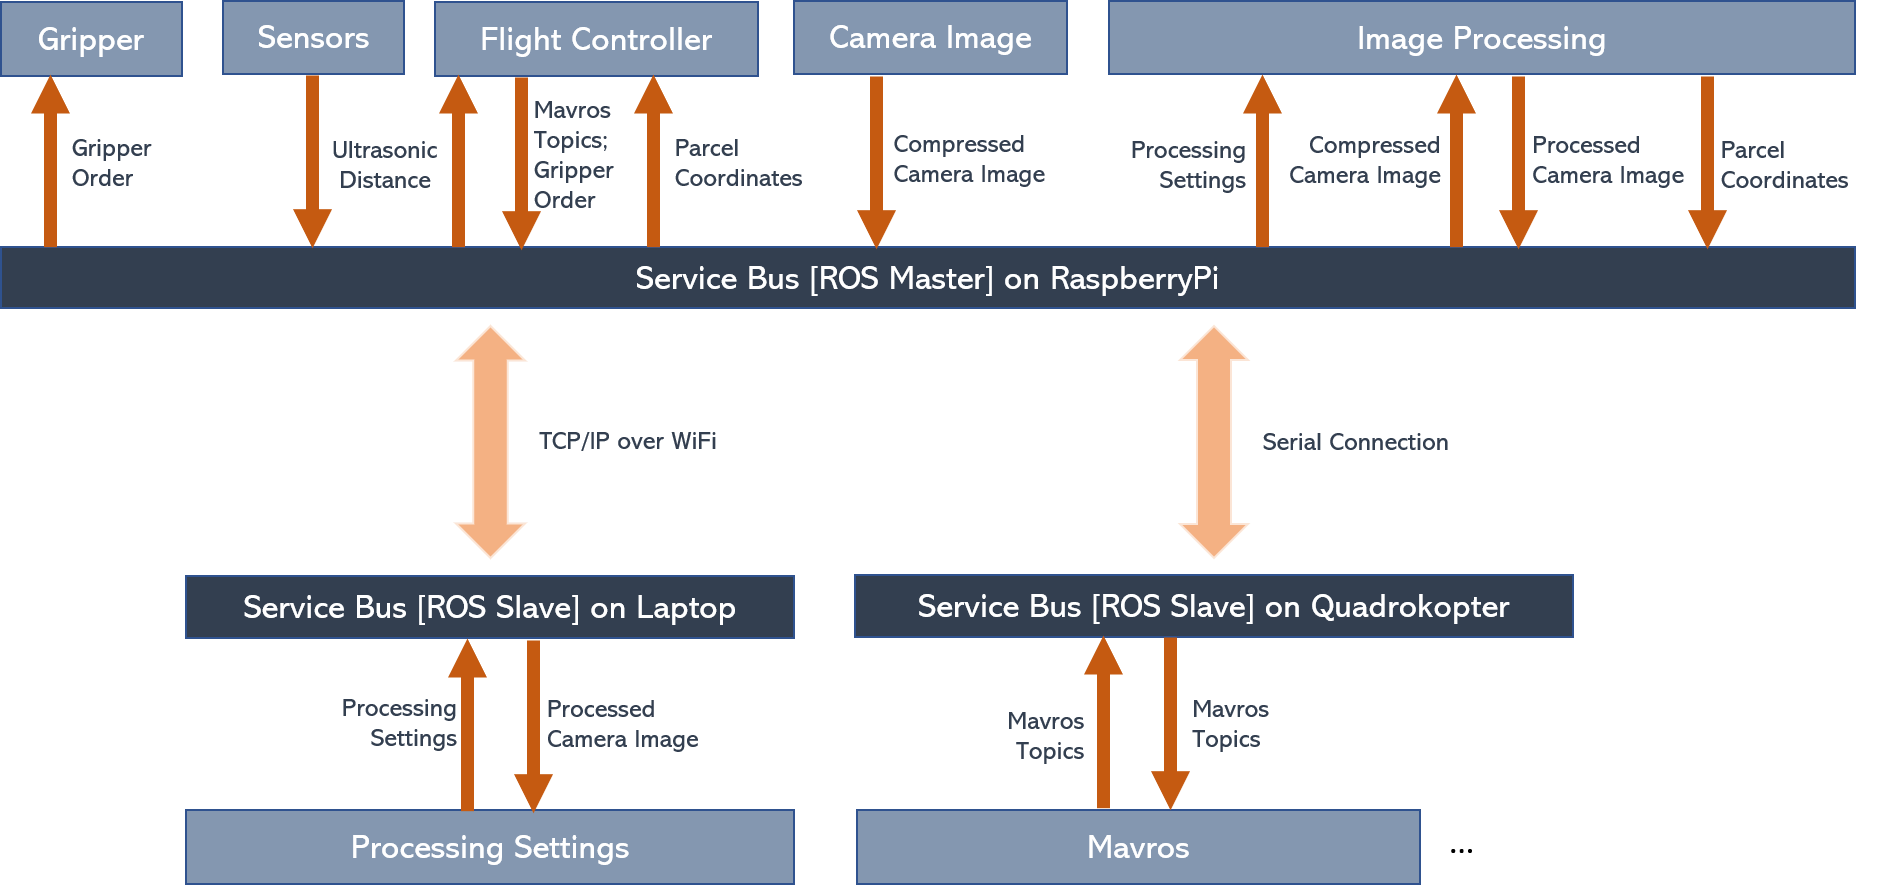
\includegraphics[scale=0.51]{"Grafiken/gesamtarchitektur.png"}
	\caption{Service Oriented Architecture}
	\label{fig:gesamtarch}
\end{figure}


\subsection{Camera Image} ist ein einfacher Publisher, der das Bild der Dronenkamera komprimiert und über den Service Bus den anderen Knoten im Netzwerk als serialisiertes numpy-Array zu Verfügung stellt. Aufgrund der später folgenden rechenintensiven Bildverarbeitung sendet dieser in der finalen Version das Bild jedoch nur mit 10 Hz. Dies is jedoch immer noch ausreichend, da sich die Geschwindigkeit der Drone nicht schnell ändern wird. 
\subsection{Image Processing} empfängt die Bilddaten von Camera Image und wir zudem über das Topic Processing-Settings vom Laptop aus konfiguriert. Dieser Knoten filtert dann das Bild um anschließend die Position und Drehung des Pakets zu ermitteln. Das gefilterte Bild und die Koordinaten als Typ
\begin{lstlisting}[language=Python]
PoseStamped
\end{lstlisting}
des Pakets werden publiziert, wobei die Z-Koordinate des 
\begin{lstlisting}[language=Python]
PoseStamped
\end{lstlisting}
die Drehung angibt.

\subsection{Sensors} Sensors verwaltet alle Sensordaten. In der aktuellen Version ist das jedoch nur der Ultraschallsensor. Die Daten werden gesammelt, aufbereitet, validiert und publiziert. So werden dann beispielsweise die Ultraschalldaten unter der Topic 
\begin{lstlisting}[language=Python]
/sensor_dist
\end{lstlisting}
im Datenformat Float32 mit einer Frequenz von 20 Hz veröffentlicht.

\subsection{Flight Controller} Flight Controller ist die zentrale Steuereinheit der neuen Funktionalität. Er empfängt alle aufbereiteten Sensordaten wie die Koordinaten des Pakets, Ultraschalldistanz, Sensordaten der Drone etc. und führt die Suche und Anflug des Pakets durch. Er gibt die Flugsteuerbefehle an Mavros über die serielle Schnittstelle weiter und gibt Greifbefehle weiter. Mehr dazu ist im Kapitel \ref{gesamtintegration} zu finden. 

\subsection{Datenübertragungsformate}
Es war sehr schwierig, die richtigen Formate zu wählen da Python im Allgemeinen eher unsauber mit den verschiedenen Datentypen umgeht. So gibt es z. B. keinen Unterschied zwischen einem 32-Bit oder einem 64-Bit Integrer. Falls die Zahl außerhalb des darstellbaren Bereiches des 32-Bit Interger liegt, so erweitert der Python-Interpreter es selbstständig zu einem 64 Bit Integer. ROS ist hingegen sehr typenspezifisch, wodurch es zuerst einige Unklarheiten bezüglich der Typen gab und diese dementsprechend verändert werden mussten.\\


\section{Implementierung der Kommunikation in ROS}
Wie bereits erwähnt basiert ROS auf dem Publisher/Subscriber Prinzip. Ein Knoten kann in ROS sowohl Publisher als auch Subscriber sein und das auch für mehrere Topics. Die Topics sind dabei hierarchisch aufgebaut und gehen vom Groben ins Feine. So publiziert beispielsweise der ``Camera Image'' Knoten das komprimierte Bild in 

\begin{lstlisting}[language=Python]
/camera/image/compressed
\end{lstlisting}. 

Anhand dieses Beispiels soll nun dargelegt werden, wie man prinzipiell bei der Erstellung eines Nodes vorgeht.


\subsection{Kamera Publisher}
Zunächst muss eine Datei mit dem Namen des Knotens und der Endung ``.py'' im entsprechenden Paketordner im src-Ordner des Catkin-Workspaces erstellt werden. Diese kann dann in PyCharm geöffnet werden, wenn nicht schon das gesamte Paket als Projekt geöffnet wurde.
Um klarzumachen, dass es sich hierbei um ein Python File handelt, muss die Datei mit 


\begin{lstlisting}[language=Python]
#!/usr/bin/env python3
\end{lstlisting}

starten, um die Pythonumgebung auszuwählen. Es folgt nun für gewöhnlich die Lizenzerklärung zur Datei. Es sollten nun 

\begin{lstlisting}[language=Python]
numpy as np, time, sys, cv2, roslib, rospy
\end{lstlisting}

importiert werden, sowie 

\begin{lstlisting}[language=Python]
CompressedImage
\end{lstlisting}aus der ROS-Bibliothek 

\begin{lstlisting}[language=Python]
sensor_msgs.msg
\end{lstlisting}. 

Es empfiehlt sich nun die gesamte Funktionalität mittels 

\begin{lstlisting}[language=Python]
def function_name
\end{lstlisting}

in eine Funktion zu packen. Dort muss dann zunächst mit 

\begin{lstlisting}[language=Python]
pub = rospy.Publisher("", DataType)
\end{lstlisting}

ein Objekt erstellt werden, wobei hier das Topic 

\begin{lstlisting}[language=Python]
"/camera/image/compressed"
\end{lstlisting}, 

sowie der Datentyp 

\begin{lstlisting}[language=Python]
CompressedImage
\end{lstlisting} 

dem Konstruktor übergeben werden müssen. Mit 

\begin{lstlisting}[language=Python]
rospy.init_node('node_name', 
	anonymous=True)
\end{lstlisting}

registriert sich der Knoten nun am ROS-Service-Bus. Nun wird die Computerbildverarbeitungsbibliothek OpenCV genutzt, um mit 

\begin{lstlisting}[language=Python]
cap = cv2.VideoCapture(0)
\end{lstlisting}

ein Objekt zu erstellen, dass auf den Datenstrom der ersten angeschlossenen Kamera zugreift. Der nun folgende Code soll so lange ausgeführt werden, wie ROS aktiv ist. Dies lässt sich mit 

\begin{lstlisting}[language=Python]
while not rospy.is_shutdown():
\end{lstlisting}

implementieren. Mit 

\begin{lstlisting}[language=Python]
ret, frame = cap.read()
\end{lstlisting}

wird nun der Datenstrom der Kamera ausgelesen und das aktuelle Bild in die Variable 

\begin{lstlisting}[language=Python]
frame
\end{lstlisting}

geschrieben. Jetzt muss mit 

\begin{lstlisting}[language=Python]
msg = CompressedImage()
\end{lstlisting}

ein Nachrichtenpaket des Typs 

\begin{lstlisting}[language=Python]
CompressedImage
\end{lstlisting}

erstellt werden, das mit 

\begin{lstlisting}[language=Python]
msg.header.stamp = rospy.Time.now()
\end{lstlisting}

um einen Zeitstempel erweitert wird und mit 

\begin{lstlisting}[language=Python]
msg.format = "jpeg"
\end{lstlisting}

das richtige Dateiformat erhält. Die Daten des Pakets werden mit der Property 

\begin{lstlisting}[language=Python]
msg.data
\end{lstlisting}

gesetzt. Diese müssen nun aus dem vorher gelesenen 

\begin{lstlisting}[language=Python]
frame
\end{lstlisting}

erstellt werden. Dafür wird zunächst mit 

\begin{lstlisting}[language=Python]
cv2.imencode('.jpg', frame)[1]
\end{lstlisting}

das 

\begin{lstlisting}[language=Python]
frame
\end{lstlisting}

mithilfe von OpenCV in ein JPEG umgewandelt und wird dann mit 

\begin{lstlisting}[language=Python]
np.array()
\end{lstlisting}

zu einem Bildarray transformiert wird und mit

\begin{lstlisting}[language=Python]
tostring()
\end{lstlisting}

serialisiert wird. Nun ist Paket bereit mit 

\begin{lstlisting}[language=Python]
pub.publish(msg)
\end{lstlisting}

an den Service Bus gesendet zu werden. Die Funktion sollte nun mit 

\begin{lstlisting}[language=Python]
if __name__ == '__main__': function_name()
\end{lstlisting}

aufgerufen werden, wobei es Sinn macht den Funktionsaufruf mit einer Ausnahmeregelung für die 

\begin{lstlisting}[language=Python]
rospy.ROSInterruptException
\end{lstlisting}

zu erweitern. 


\subsection{Kamera Subscriber}
Der dazugehörige Subscriber ist im Knoten ``Image Processing'' implementiert und ist dem Publisher gegenüber recht ähnlich aufgebaut. Hier wird jedoch ein Subscriber-Objekt mit 

\begin{lstlisting}[language=Python]
rospy.Subscriber("topic", 
	DataType,
	callback)
\end{lstlisting}

erstellt, wobei callback die Callback-Funktion ist, die aufgerufen wird, wenn eine neue Nachricht in der Topic ankommt. In den Argumenten dieser Funktion eine Variable 

\begin{lstlisting}[language=Python]
msg
\end{lstlisting}

definiert sein, in der die Nachricht bei Empfang gespeichert wird. Der Inhalt der Nachricht kann mit 

\begin{lstlisting}[language=Python]
msg.data
\end{lstlisting}

aufgerufen werden und mit 

\begin{lstlisting}[language=Python]
np.fromstring(data, np.uint8)
\end{lstlisting}

zuerst zu einem 

\begin{lstlisting}[language=Python]
numpy
\end{lstlisting}-Array deserialisiert und dann mit 

\begin{lstlisting}[language=Python]
cv2.imdecode(np_arr, cv2.IMREAD_COLOR)
\end{lstlisting}

zu einem für OpenCV verarbeitbarem Format dekodiert werden. Der darauf folgende Code zur Bildverarbeitung ist in Kapitel \ref{bilderkennung}. beschrieben. 
\cite{aniskoubaa2019}

\section{Starten und Automation eines ROS-Systems}
Damit die Knoten auch lauffähig sind, müssen die Dateien zunächst mit 

\begin{lstlisting}[language=bash]
chmod +x
\end{lstlisting}

für den Kernel ausführbar gekennzeichnet werden. Nun können, nachdem 

\begin{lstlisting}[language=bash]
roscore
\end{lstlisting}

ausgeführt wurde, in einem jeweils neuen Terminaltab mit 

\begin{lstlisting}[language=bash]
rosrun paketname knotenname.py
\end{lstlisting}

die verschiedenen Knoten ausgeführt werden. Mit 

\begin{lstlisting}[language=bash]
rostopic echo /topic/name
\end{lstlisting}

können die Nachrichten der verschiedenen Topics überwacht werden. Um das alle nicht jedes Mal von Hand machen zu müssen, gibt es bei ROS sogenannte Launch-Files, die, wenn ausgeführt, nicht nur einen ROS-Core ausführen, sondern auch alle notwendigen Knoten startet, Umgebungsvariablen setzt etc. Das Launch File basiert auf XML und enthält innerhalb des 

\begin{lstlisting}[language=xml]
<launch></launch>
\end{lstlisting}Tags alle Komponenten. Ein Knoten ist dabei recht selbsterklärend aufgebaut: 

\begin{lstlisting}[language=xml]
<node name="CameraImagePub" 
	pkg="parcelcopter" 
	type="CameraImagePub.py"/>\end{lstlisting}

Innerhalb des Tags können außerdem Startparameter mit 

\begin{lstlisting}[language=bash]
arg
\end{lstlisting}

definiert werden.Mit dem 

\begin{lstlisting}[language=bash]
env
\end{lstlisting}-Tag können zudem Umgebungsvariablen gesetzt werden.

Man bemerke hier die Modularität und Stabilität von ROS. Denn die Knoten geben keinen Fehler aus, obwohl ein anderer Knoten, der eigentlich für die Ausführung von Nöten ist, noch gar nicht gestartet ist. Sobald dieser bereit ist, fangen die davon abhängigen Knoten automatisch an zu arbeiten. 

\section{Mavros und Simulation}
Die Simulation der Drohne erfolgt in Gazebo. Dafür wird ein PX4-Controller simuliert. Gazebo greift die Signale von dem ROS Interface ab und verarbeitet sie. Dafür wird eine FPL-Drohne simuliert. Ihre Daten sendet dann Gazebo wieder an den PX4-Controller. Weiterhin sendet es einen Video-Stream mit den simulierten Bildern. Dieser wird dann von der Node ImagePub erkannt und in ROS gestreamt. Eigentlich kommt er schon über ROS aber auf diesem Wege ist es realitätsgetreuer. (Die Alternative wäre einfach eine andere Quelle für den ImagePub anzugeben.) Auf diesem Wege kann die Drohne nahezu eins zu eins simuliert werden. \\
\\
Auf diesem Wege wurden bereits viele Fehler wie z. B. Vorzeichenfehler bei den Berechnungen gefunden. Jedoch ist es etwas kompliziert neue Drohnen zu implementieren, da dies erst die Umgebung programmiert werden muss. Unten sieht man einen Kurzfilm, welcher eine Simulation zeigt.
\\
Auch bei der Simulation ist ROS von Vorteil, da man im Testmodus einfach einen Sensor simulieren kann ohne die eigentlichen funktionsverarbeitenden Programme umschreiben zu müssen. Diese Programme laufen dann auf einem externen PC, der sich im gleichen Netzwerk wie die der Pi befindet, und senden regelmäßig ``Fake'' Nachrichten (auch als Fake News) bekannt.
Außerdem kann man so über einen externen PC einfach den Datenfluss kontrollieren, da man quasi die Rohdaten abrufen kann, um die Funktion der einzelnen Programme zu überprüfen. Das ist natürlich auch ein gewisses Sicherheitsrisiko, weshalb die eingehende Kommunikation in den Service Bus beispielsweise durch ein sicheres WiFi-Netzwerk restriktiert werden muss. 

	\chapter{Bilderkennung}
\label{bilderkennung}
Bei dem Bildverarbeitungsprozess muss das Paket vor verschiedenen Hintergründen, erkannt werden. Dabei darf die Beleuchtung keine Rolle spielen. Die charakteristischen Eigenschaften sind neben Farbe somit ebenfalls Form und Größe.

Zuerst wurde RGB(Red, Green, Blue) Farbraum gefiltert. Jedoch ergaben Test's das der RGB-Farbraum sehr belichtungsempfindlich ist. Deswegen wird das Bild in den HSV(Hue, Saturation, Value) Farbraum konvertiert. Dieser ist deutlich belichtungsstabiler.
\begin{figure}[h]
	\begin{center}
	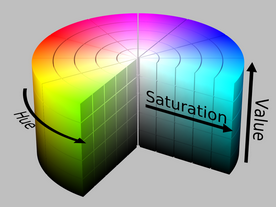
\includegraphics[scale=0.5]{"Grafiken/hsv_colorspace_zoom34.png"}
	\caption{HSV-Raum\protect\footnotemark}
	\label{fig:meine-grafik}
	\end{center}
\end{figure}
\footnotetext{Quelle: http://www.subcolors.de/content/public/colorsystems/rgb.html  }

Als Farbe wäre Rot sehr geeignet, da es in unsere Umgebung sehr selten vorkommt. Allerdings gibt es keine Roten-Pakete. Außerdem ist Rot für eine Kamera sehr schwer zu erkennen, da es eine der Grundfarben ist und damit in fast jeder Farbe vorkommt. Deswegen wurde als Farbe weiß gewählt. Durch den Filter werden nun weiße Flächen weiß und der Rest wird schwarz. Da das Experiment auf einem dunklen Boden stattfindet, bietet sich dies an.

Weiterhin muss auf dem Paket mittig, ein weiteres schwarzes Viereck sein. Dies ist nötig um eine Orientierung bei naher Distanz zu gewährleisten. Befindet sich die Drohne nahe über dem Paket, so füllt es das komplette Kamerasichtfeld aus. Um sich nun orientieren zu können ist ein weiteres Viereck nötig. Dies muss mittig sein, da sich die Drohne im Verlauf des Anflugs parallel zu dem Rechteck ausrichtet. Damit bei allen Rotationen der Versatz immer gleich ist, muss es mittig sein. Dadurch kann man ihn in der Kameraregelung berücksichtigen.

Für die Form wird der Hought-Transformation verwendet. Bei dieser wird das Bild zuerst abgeleitet. Also werden Pixel neben den sich ein andersfarbiges befindet weiß und der Rest(Weiß neben Weiß, Schwarz neben Schwarz) wird schwarz. Nun sind die Kanten deutlich zu sehen. Anschließend wird durch jeden weißen Punkt eine Linie mit verschieden Anstiegen zwischen - unendlich und + unendlich gelegt. Schneidet man dabei mit der Linie einen anderen weißen Punkt, so wird sich diese Linie gemerkt. Linien, die durch mehrere weiße Punkte gehen werden, so als Linien detektiert. Der Algorithmus wird aus der OpenCV Bibliothek implementiert. Er hat die Komplexität: n! (n Fakultät). \cite{wenyu2007}

Anschließend wird das Bild nach Konturen durchsucht. Dabei sind nur die Konturen mit 4 Ecken von Bedeutung. Diese Konturen werden nun nach minimaler und maximaler Größe gefiltert. Die Intervallbreite variiert abhängig von der Flughöhe. Außerdem spielt die Auflösung der Kamera ein Rolle, diese ist 640*480p (\ref{kamera})

Von den gefilterten Rechtecken wird nun der Mittelpunkt berechnet. Ist mit einem Umkreis von 10 Pixeln bereits ein weiteres Rechteck gefunden worden, so wird das Rechteck verworfen. Dadurch ist sicher gestellt, dass Rechtecke nicht doppelt erkannt werden. Erfüllt ein Rechteck all diese Bedingungen so wird noch die Rotation der oberen Kante berechnet. Diese wird dann zusammen mit den Mittelpunktkoordinaten an den Controller über ROS weitergeleitet. Es ist das Problem aufgetreten, dass das Viereck um 45° gedreht war. In diesem Fall gibt es 2 oberste kanten und der Algorithmus erkennt schlimmstenfalls abwechselnd beide. Um dies zu vermeiden, wurde eine 2 Regel eingeführt. Es wir immer die oberste Kante genommen. Gibt es 2, so wird die Linke davon genommen. Da es nicht 2 Oberste und Linkeste geben kann, ist der Algorithmus so eindeutig definiert und terminiert.\cite{Lagunovsky1997}

Um die Rechenzeit zu verringern, wird das Bild auf 640x480 Pixel herunter skaliert, da dies für einfache Vierecke völlig ausreicht. Außerdem wird der Hough Algorithmus bewusst erst nach dem Filtern ausgeführt, da seine Komplexität fakultativ mit der Anzahl der erkannten Objekte ansteigt. Auf diesem Wege ist eine Auswertung mit mehr als 5 Frames pro Sekunde möglich, was unseren Anforderungen genügt.

Der Bildverarbeitungsprozess läuft in der Image Progressing Node. Er wird maximal mit 10 Hz ausgeführt. Das stellt sicher das der Pi nicht überlastet und noch genügend Rechenkapazität für die anderen Codes/Prozesse hat. Da die Drohne nicht zu schnell fliegt, reicht dieses Schrittweite aus um ein stabiles Systemverhalten des PT1-Glied(Regler mit proportionaler Vergrößerung erster Ordnung). Es wurde experimentell in der Gazebosimulation herausgefunden das bei dem PX-4 Controller sogar eine Geschwindigkeit von 3 HZ ausreichend würde, da die Änderungsraten klein sind 0.1. Diese 0.1 steht dafür das, wenn der Regler eine Abweichung von 1 m erkennt, er der Drohne als neue Zielkoordinaten nur Koordinaten gibt, die 0,1 m entfernt sind. Dadurch fliegt sie langsamer und kippt nicht so stark. Durch das kippen wird die Kamera bewegt und ändert somit ihren Winkel auf den Boden. Dadurch wiederum wird das Paket falsch erkannt. (siehe Kapitel \ref{fazit}) 
	\chapter{Gesamtintegration}
\label{gesamtintegration}
%\section{Programmaufbau}
%\begin{figure}[h]
%	\centering
%	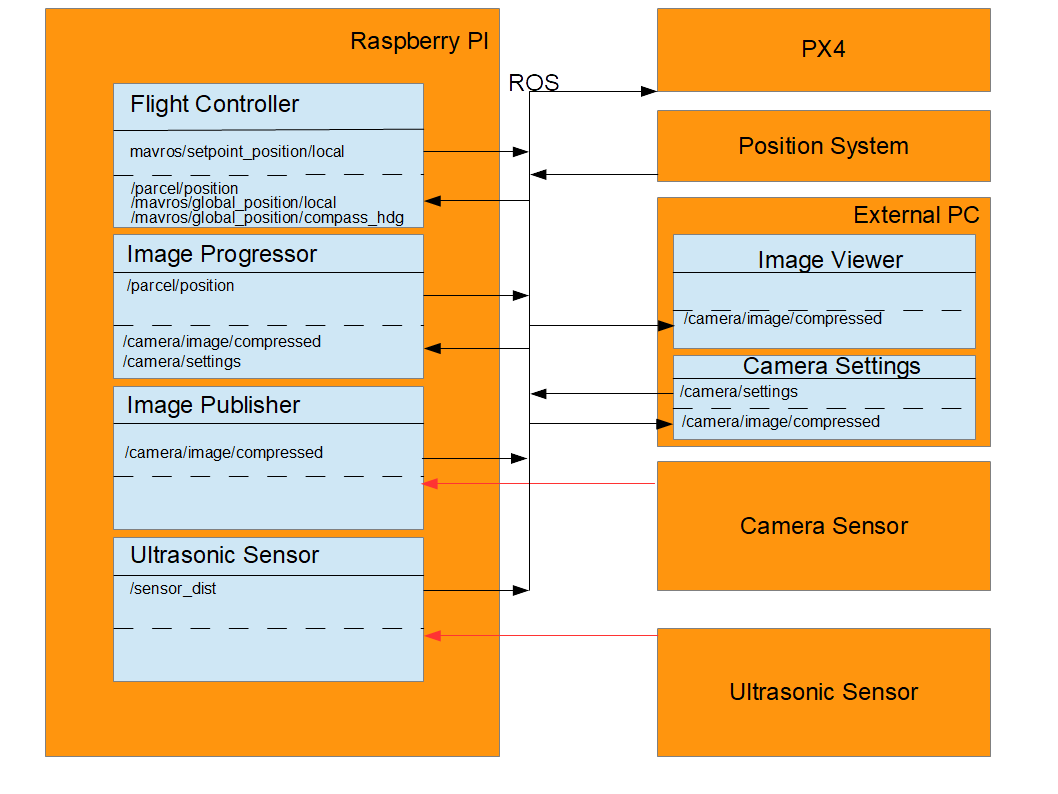
\includegraphics[scale=0.5]{"Grafiken/Nodes.png"}
%	\caption{Programmaufbau}
%	\label{fig:meine-grafik}
%\end{figure}
%Das Programm besteht grundlegend aus 4 Nodes/Unterprogrammen. Zum einen dem Image Publisher und Ultrasonic Sensor. Und zum anderen aus dem Image Progressor und Flight %Controller, um diese Daten zu verarbeiten. In der obigen Grafik sind diese Nodes, sowie deren empfangene(unten) und gesendete(oben) Themen zu sehen. \\
%\\
%Alle 4 Nodes laufen gleichzeitig und kommunizieren über das Interface ROS(siehe Interfaces). Um Multithreading(ein paralleles ablaufen der Unterprogramme) zu gewährleisten, wird jedes Programm in einem separaten Thread ausgeführt.\\
%\\
%Grundlegend sind alle Programme gleich aufgebaut. Zuerst gibt es einen Teil, der die Verbindung zum ROS Interface herstellt. Dafür wird zuerst gewartet, bis der Server läuft, anschließend werden die entsprechenden Themen deklariert. Nun geht das Programm in eine Schleife, bei der es auf eine ankommende Nachricht wartet. Empfängt es eine Nachricht, so verarbeitet es diese. Gegenbefalls sendet es regelmäßig eine neue Nachricht. Der Server auf dem diese Themen laufen, wird dabei vom Raspberry Pi gehostet. Sobald dieser steht, können alle Nodes zu spezifischen Themen Nachrichten senden oder die gesendeten Nachrichten zu diesen Themen empfangen.\\
%\\

\section{Sensordatenverarbeitung}
Prinzipiell gibt es 3. Sensoren. Zum einen der Ultraschallsensor, um die Höhe genau und jederzeit bestimmen zu können. Außerdem gibt es einen Kamerasensor, um die Position des Paketes zu bestimmen. Das dritte Sensorsystem ist da, um die Position der Drohne zu bestimmen. Dieses wird vom Institut für Technische und Numerische Mechanik gestellt. Es ist für das fliegen der Drohne existenziell wichtig.

Leider ist ein Fliegen der Drohne ohne dies nicht möglich, weil die Drohne mit globalen Koordinaten arbeitet. Das heißt, dass System bestimmt die Position der Drohne im Raum, anschließend berechnet der Flight Controller die nächste Sollposition und schickt sie an den PX4-Controller. Dieser regelt dann seine Lage dem entsprechend. Der Vorteil an diesem Vorgehen ist, dass die Drohne leicht auf eine externe Positionsbestimmung(z. B. GPS) umgestellt werden kann. 
Mit dem Ultraschallsensor ist eine genaue Höhenbestimmung immer noch möglich. Der Nachteil ist, dass man die Drohe ohne das System nicht fliegen kann. Die Umstellung auf GPS oder Galileo wäre z. B. ein denkbares Folgeprojekt. Mehr dazu ist unter Auswertung und Fazit zu finden.

Ein weiteres wichtiges Merkmal ist die Einheit der Sensordaten. Zu dem der Ultraschallsensor liefert dabei sein Ergebnis in mm. Näheres dazu findet man unter dem Kapitel ``Sensorik, Aktorik und andere Hardware''.

Die Kamera bestimmt die Bildposition in Pixel. Abhängig vom Öffnungswinkel der Kamera ist die Position des Paketes daraus zu berechnen.
Die Formel für die $x$/$y$~-Koordinate ist:
\begin{equation}
\begin{split}
x = \frac{x^*}{a^*} \tan(\frac{a}{2}) h\\
y = \frac{y^*}{b^*} \tan(\frac{b}{2}) h\\
\end{split}
\end{equation}
wobei:\\
a/b* = Bildpunkte in x/y Richtung\\
x/y* = erkannte Punkte\\
a/b = Öffungswinkel\\

\begin{figure}[h]
	\centering
	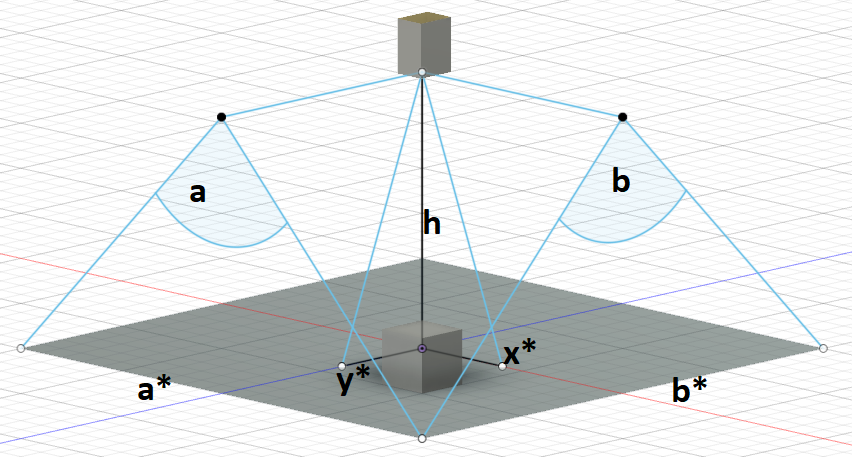
\includegraphics[scale=0.3]{"Grafiken/Kameraformel.png"}
	\caption{Kamerawinkel}
	\label{fig:kameraformel}
\end{figure}
\section{Programmablauf}
Prinzipiell ist jede Node gleich aufgebaut. Zuerst gibt es eine Initialisierung und Verbindung mit der Masternode. Anschließend deklariert die Node welche Streams die entsprechende Node benötigt und welche nicht. Nun wird gewartet, bis eine neue Nachricht auftaucht und die diese wird dann verarbeitet. Geprüft wird in diesem Fall mit einer Rate von 20 Hz. 

Der Flight-Controller verhält sich jedoch leicht anders. Die PX-4 muss erst in den Offboard-Modus versetzt werden. Dieser bedeutet, dass die Drohne extern gesteuert werden kann. Außerdem muss der Arming-Modus aktiviert werden. Damit sie Befehle annimmt. Leider hat das einmalige Senden nicht gereicht. Sie hat nicht zuverlässig beide Befehle erkannt. Damit dies gewährleistet ist, sendet der Pi nun aller 5 Sekunden den Offboard Befehl, solange bis sich der Status der Drohne geändert hat, sodass sie sich nun im Offboardmodus befindet. Anschließend sendet der Controller das Arming Signal, solange bis die Drohne sich im Arming Modus befindet.

Wichtig ist das gleichzeitig mit 20 Hz, eine Sollposition gesendet werden muss, damit die Drohne im nicht wieder aus dem Offboardmodus geht. Dies hat am Anfang große Probleme bereitet, da man so schnell die Kontrolle verliert.

Anschließend wird zuerst eine Sollposition angeflogen. Aus dieser Position muss die Drohne, das Paket sehen. Die Abbildung \ref{fig:Drone_Simulation1} zeigt links oben das gefilterte Bild, links unten das Bild der Kamera mit dem erkannten Paket und rechts ein Bild der Drone in der Simulation. 


 Anschließend richtet sich die Drohne mithilfe der Kamera mittig über dem Paket aus. Dabei vergleicht der Kontroller die aktuelle Position mit der Paketposition. Die Paketposition wird dabei mithilfe der Formel(siehe Sensorerfassung) berechnet. Um keine zu schnellen Änderungen zu fliegen wird ein P-Regler verwendet. Ist das Paket mittig und die Drohne nicht zu schnell(dies wird mithilfe der alten Position und der neuen Position bestimmt) so sinkt die Drohne. Hat sie eine Höhe von 60 cm erreicht, so dreht sie sich und richtet sich entlang des Paketes aus. Dabei verfährt sie nach dem gleichen Verfahren wie bei der Positionsausrichtung und wartet immer, bis das Paket wieder mittig ist. Siehe Abb. \ref{fig:Drone_Simulation2}

 Ist die Verdrehung kleiner als 3 Grad, sinkt sie weiter. 
 
   Ist sie nur noch 20 cm über dem Boden, so hat sie das Paket gefunden und schließt den Greifer. Anschließend könnte sie wieder abheben und das Paket zur Zielposition bringen. Der Prozess ist in dem unteren Strukturgramm Abb. \ref{fig:Programmablauf} dargestellt. In der Simulation hält sie ihr Position weiterhin. Siehe Abb, 
\begin{figure}[h]
	\centering
	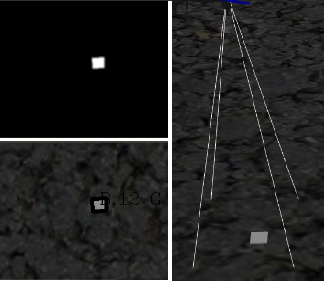
\includegraphics[scale=1.3]{"Grafiken/Drone_Gazebossimulatiuon1.png"}
	\caption{Simulation der Drohne}
	\label{fig:Drone_Simulation1}
\end{figure}

\begin{figure}[h]
	\centering
	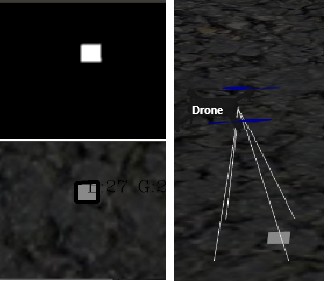
\includegraphics[scale=1.3]{"Grafiken/Drone_Gazebossimulatiuon2.png"}
	\caption{Ausrichten über dem Paket}
	\label{fig:Drone_Simulation2}
\end{figure}

\begin{figure}[h]
	\centering
	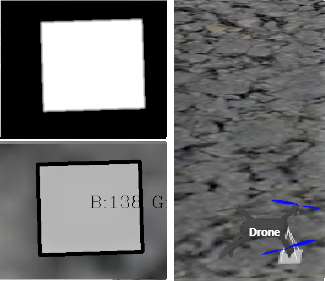
\includegraphics[scale=1.3]{"Grafiken/Drone_Gazebossimulatiuon3.png"}
	\caption{Halten der Position}
	\label{fig:Drone_Simulation3}
\end{figure}

\begin{figure}[h]
	\centering
	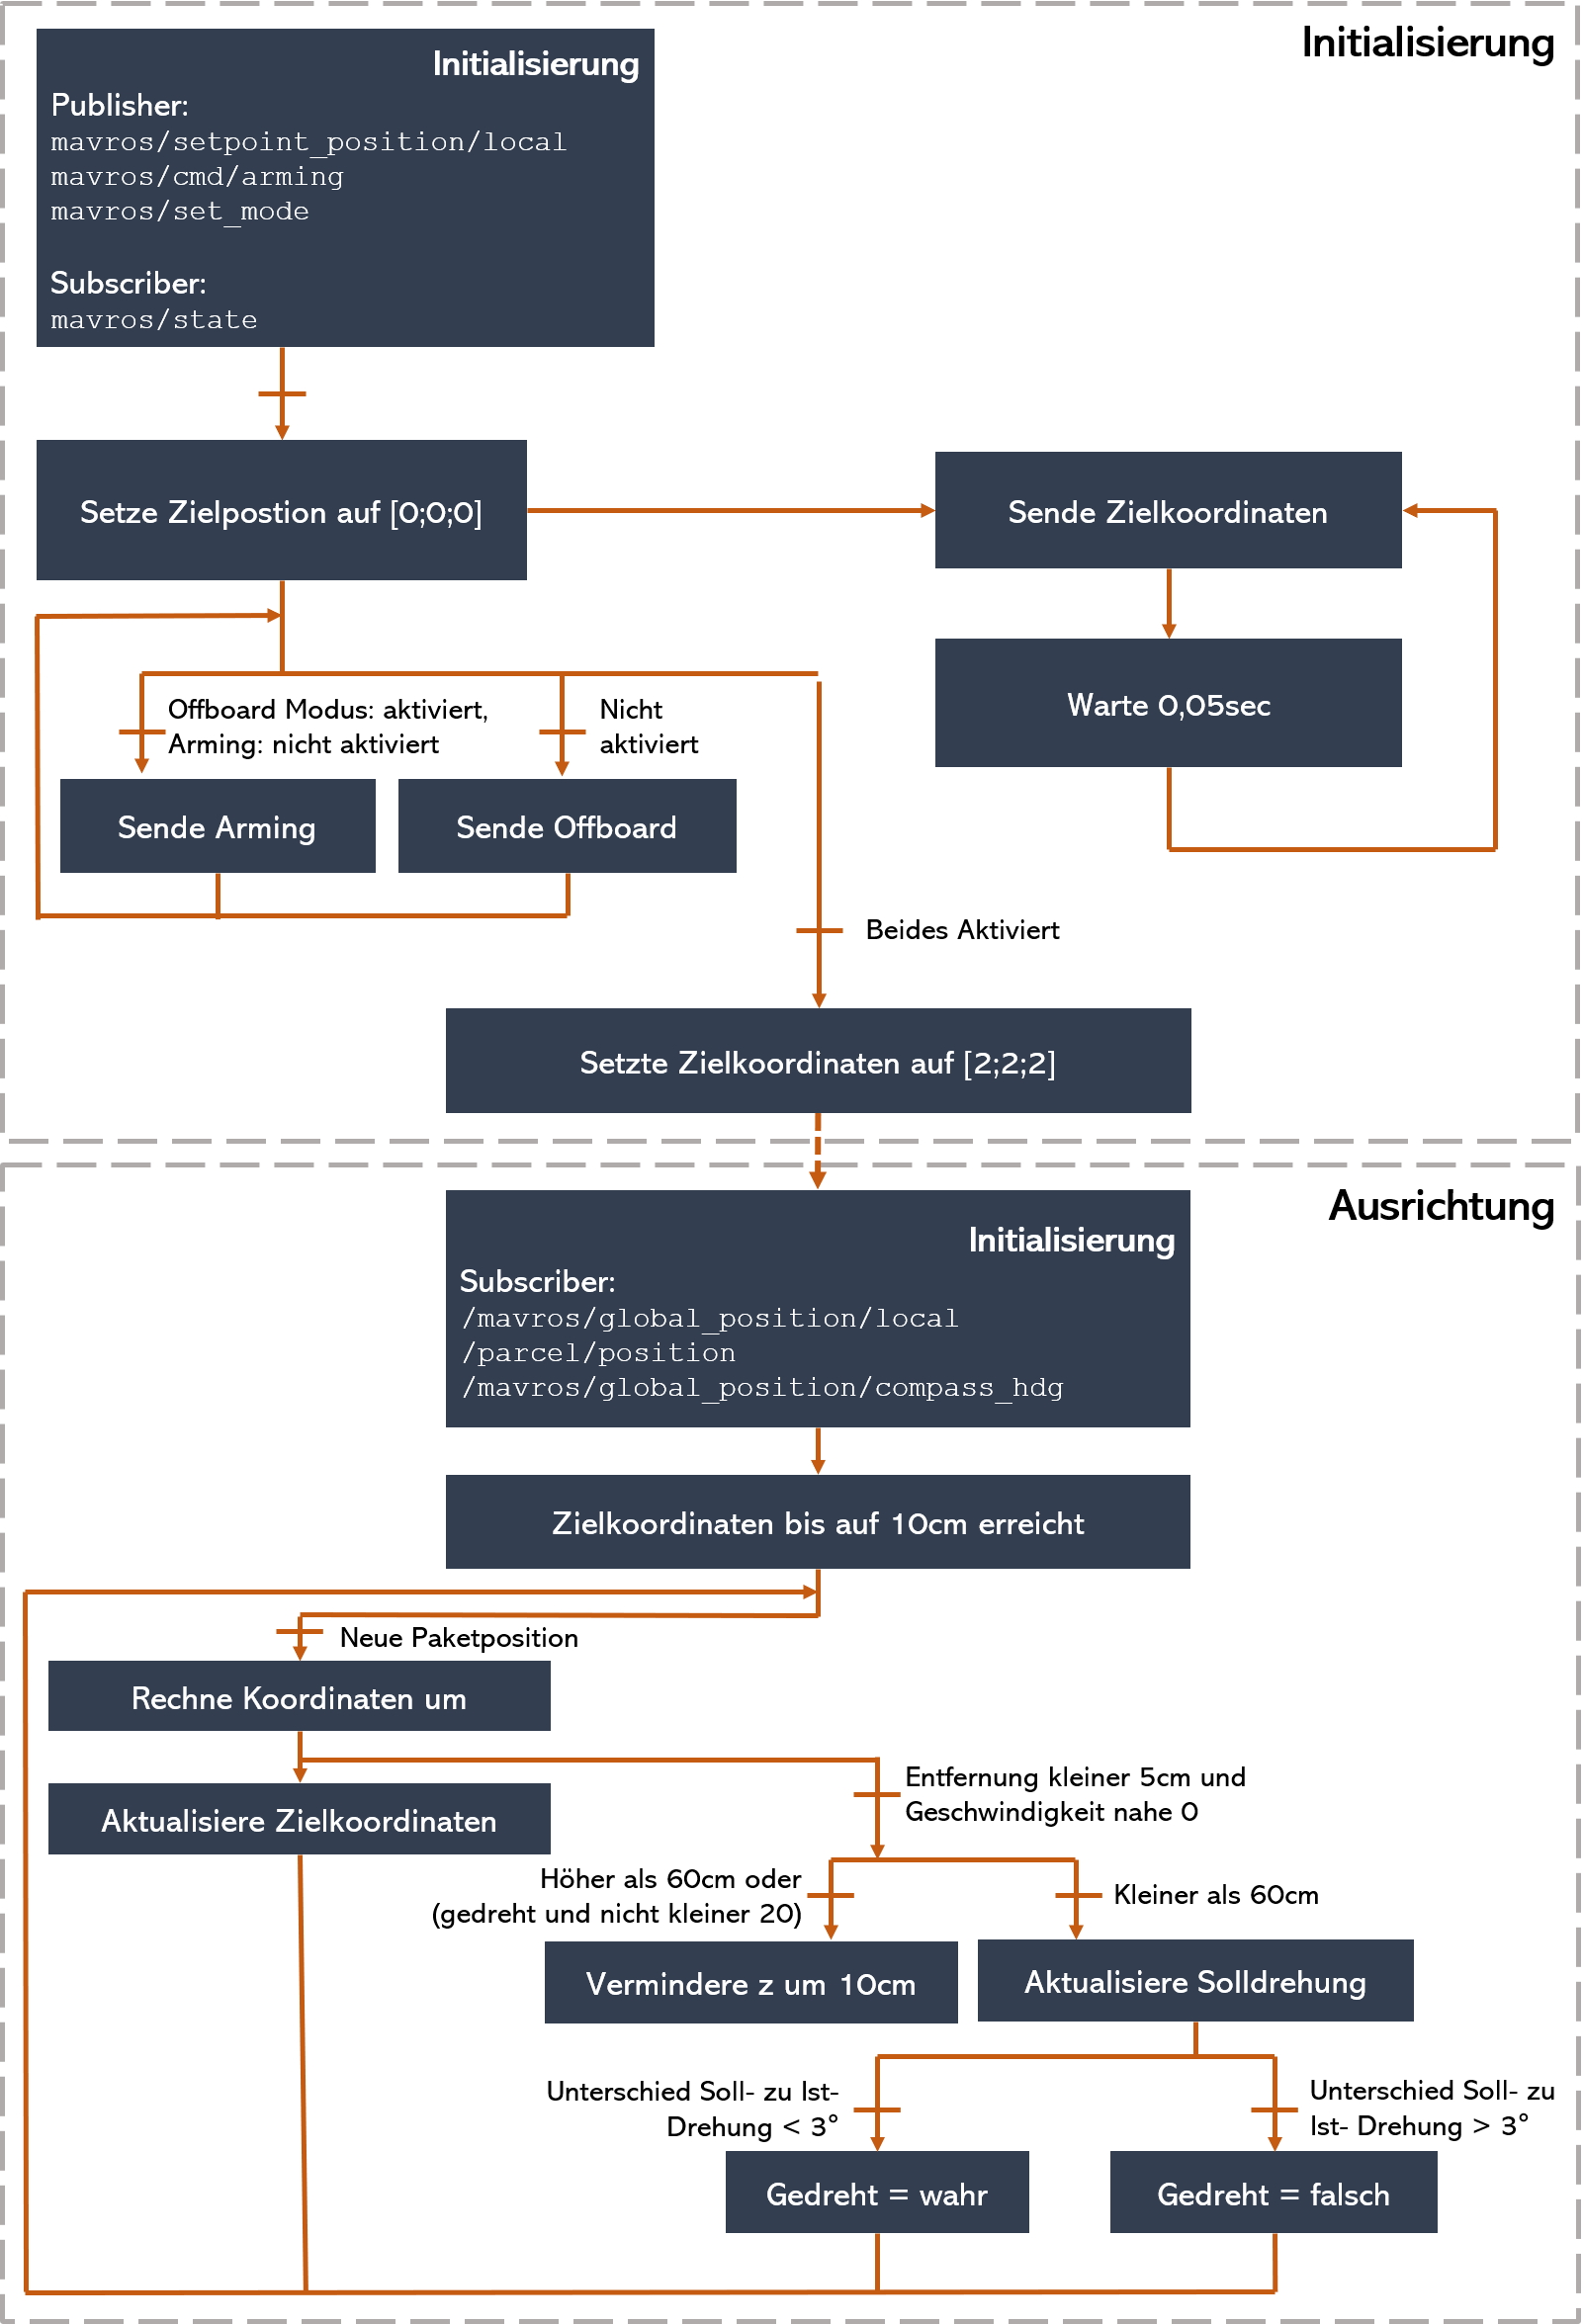
\includegraphics[scale=0.5]{"Grafiken/Prozellablauf.png"}
	\caption{Funktionsablaufdiagramm}
	\label{fig:Programmablauf}
\end{figure}
	\chapter{Fazit und Ausblick}
\label{fazit}
Zusammengefasst ist zu erkennen, dass eine Drohnenregelung durchaus auch mit einfachen Mitteln machbar ist. Besonders überraschend war jedoch, dass die Bilderkennung nicht so gut funktioniert wie gedacht. Es ist sehr schwierig einzelne äußere Faktoren zu Eliminieren und immer zu dem „richtigen“ Ergebnis zu kommen. Jedoch funktioniert das Ansteuern des PX-4 Controllers erstaunlich problemlos. Es hat uns große Schwierigkeiten bereitet die Umgebung zu installieren da diverse Packages manuell nachinstalliert werden müssen. Gerade den Catkin-WS zu erstellen und in diesem die richtigen Pakete zu installieren hat sehr viel Zeit in Anspruch genommen.
In den nächsten Wochen wollen wir die Software dann vollständig integrieren und testen. Wenn diese Test's erfolgreich verlaufen so ist die Projektarbeit damit abgeschlossen.\\
\\
Trotzdem bleiben einige Themen leider offen. Vielleicht für nachfolgende Gruppen.
Die größten softwareseitigen Probleme sind zum einen die Bilderkennung, dort wären mögliche Lösungsansätze das Auslagern des Prozesses der Bilderkennung. Dadurch könnte massiv Laufzeit gewonnen werden, weil dieser Anspruchsvolle teil auf einem Externen leistungsfähigeren Rechner gemacht werden könnte. 
Weiterhin könnte die Bilderkennung dahin verbessert werden das zusätzliche starke Lampen an der Unterseite befestigt werden, um das Paket bei verschiedenen Belichtungen erkennen zu können.\\
Ein weiterer Punkt ist das Herausrechnen des Drohnenwinkels bei der Bestimmung der Position. Der Vorteil dabei wäre, dass man deutlich schneller fliegen könnte, da die Drohne sich mehr neigen könnte.\\
\\
Insgesamt könnte noch einiges an Laufzeit gewonnen werden, indem man Prozesse beschleunigt, jedoch sind dafür ausführliche Test notwendig.
Am Anfang des Projektes war es angedacht ein GPS-Modul zu integrieren, um die Drohne auch draußen fliegen zu können. Leider ging dies Sicherheitsbedingt nicht. Trotzdem wäre es sinnvoll, da der Einsatz der Paketdrohne erst draußen richtig sinnvoll ist.\\
\\
Trotz aller dieser Punkte die noch Fehlen, ist der Parcelcopter ein gutes Stück weiterentwickelt worden. Sowohl Hardware technisch mit einem neuen Greifer als auch Softwareseitigen mit einer Bilderkennung und Drohnensteuerung.\\
\\

	
	
	
	\bibliographystyle{itm_studdidipl_deu}
	% \bibliographystyle{/home/itm/institut/latex/Styles/BibTex/itm_phd_deu}
	%\bibliography{/home/itm/institut/Vorlagen/Latex_Vorlagen/ITM_Literatur/ITM_Literatur,Eigene_Literatur}
	%\include{QuadroLiteratur}
	\bibliography{QuadroLiteratur}
	
	
%###########################################################################
%
%   Anhang
%
%###########################################################################
\begin{appendix}
\chapter*{Anhang}
\setcounter{chapter}{1}
\addcontentsline{toc}{chapter}{Anhang}

%###########################################################################
%   Anhang A
%###########################################################################
\section{ROS auf Ubuntu}
Für eine effektive und effiziente Entwicklung des Softwaresystems ist die Nutzung geeigneter unterstützender Software unabdingbar. Daher soll nun die verwendete Toolchain kurz vorgestellt werden.
\subsection{Setup}
\markboth{Anhang}{Anhang}
Sowohl die Entwicklung als auch die Runtime läuft auf Ubuntu 18.04. Das gilt also sowohl für Entwicklungsrechner, als auch für den Raspberry Pi, wobei bei diesem Ubuntu Mate eingesetzt wird. Der Vorteil ist, dass ROS nativ darauf funktioniert und sehr viele Bibliotheken für ROS bereits vorkompiliert zur Verfügung stehen. Es ist dabei für die aktuelle ROS-Version "Melodic" dringend davon abzuraten, das System auf einer Raspian-Installation laufen zu lassen, da man einerseits alle Pakete selber kompilieren muss und darüber hinaus viele der Abhängigkeiten von MAVROS nicht zu Verfügung stehen. Wichtig ist auch, dass "Melodic" ausschließlich von der Ubuntu-Version 18.04 unterstützt wird. Die Installation von ROS lässt sich auf Ubuntu nach Hinzufügen des Repositories über 

\begin{lstlisting}[language=bash]
$ sudo apt install ros-melodic-ros-base
\end{lstlisting}

einfach durchführen. Hierbei ist es empfehlenswert für den Raspberry Pi die 

\begin{lstlisting}[language=bash]
$ ros-base
\end{lstlisting}

Version und für den Entwicklungsrechner die 

\begin{lstlisting}[language=bash]
$ desktop-full
\end{lstlisting}

Version zu nehmen, da diese bereits die wichtigsten grafischen Werkzeuge installiert hat. Nachdem man nun noch rosdep initialisiert, welches das Arbeiten mit Softwareabhängigkeiten deutlich vereinfacht, müssen nun die mitinstallierten ROS-Pakete im aktuell genutzten Terminal mit Hilfe des 

\begin{lstlisting}[language=bash]
$ source
\end{lstlisting}

Befehls geladen werden. Bei einer Standardinstallation geht das mit 

\begin{lstlisting}[language=bash]
$ source /opt/ros/melodic/setup.bash
\end{lstlisting}. \cite{martinez2013learning}

%###########################################################################
%    Anhang B
%###########################################################################
\subsection{Workspaces}
\markboth{Anhang}{Anhang}
Alle eigenen Entwicklungen finden im sogenannten catkin-Workspace statt, worin sich die eigenen Pakete befinden. Dieser kann im home-Verzeichnis des Benutzers nach Erstellen des Verzeichnisses "catkin\_ws" mit 

\begin{lstlisting}[language=bash]
$ catkin_make 
-DPYTHON_EXECUTABLE
=/usr/bin/python3
\end{lstlisting}

erstellt werden. Dabei muss 

\begin{lstlisting}[language=bash]
$ catkin_make
\end{lstlisting}

jedes mal ausgeführt werden, wenn ein neues Paket erstellt wurde. Das kann mit dem Befehl 

\begin{lstlisting}[language=bash]
$ catkin_create_pkg my-package-name 
std_msgs rospy roscpp
\end{lstlisting}

erreicht werden. Dadurch wir ein gleichnamiger Ordner im ``src''-Ordner des Workspaces erstellt, in dem die Sourcedateien abgelegt werden können. Um die neuen Pakete nun auch in ROS zu Verfügung zu haben, müssen diese auch im Terminal geladen werden. Das geht analog zum Laden der vorinstallierten Pakete mit 

\begin{lstlisting}[language=bash]
$ source ~/catkin_ws/devel/setup.bash
\end{lstlisting}.

\subsection{.bashrc}
\markboth{Anhang}{Anhang}
Um nicht bei jedem neuen Terminal erst die Pakete manuell laden zu müssen, bietet Ubuntu die Möglichkeit dies automatisch zu tun. Dafür ist die Datei .bashrc zuständig, die sich im home-Verzeichnis eines jeden Benutzer befindet. In diese können die beiden Befehle einfach angehängt werden. Auch die Konfiguration für Gazebo (siehe Kapitel \ref{gesamtintegration}) kann hier bereits erfolgen. Es sei aber zu erwähnen, dass dies nur so lange sinnvoll ist, wie ROS hauptsächlich auf dem System genutzt wird. 

\section{Entwicklungsumgebung und Versionsverwaltung}
\markboth{Anhang}{Anhang}
Eine (integrierte) Entwicklungsumgebung sollte den Entwickler in seiner Arbeit unterstützen und ihm sich wiederholende oder logisch einfache, aber zeitaufwändige Schritte abnehmen. Für diese Entwicklung fiel daher die Wahl auf "PyCharm" der Firma JetBrains. Dieses bietet neben dem obligatorischen Texteditor mit integriertem Auto-Complete und Compiler Vorschläge zu Codeverbesserung Refactoring etc. Es macht hier jedoch Sinn sich eine der ROS-Erweiterungen für PyCharm zu installieren, damit die ROS-eigenen Python Bibliotheken auch korrekt erkannt werden. PyCharm arbeitet zudem mit Virtual Environments (venv), also einer abgekapselten, meist projektspezifischen Python-Installation, die nur die zusätzlichen Bibliotheken enthält, die für das aktuelle Projekt benötigt werden. Diese sollte bei allen Entwicklern identisch sein, um Versionsinkompatibilitäten zu vermeiden. Ein weitere Funktion von PyCharm ist die integrierte Versionsverwaltung, kurz VCS (Version Control System). Diese bietet eine direkte Anbindung an Git, das Versionen des Sourcecodes verwaltet und Teilentwicklungen in den verschieden Entwicklungszweigen (branch) der Entwickler effektiv zum Hauptzweig (master) zusammenbringt (merge). Konflikte, wenn beispielsweise eine Datei von zwei zu vereinenden Zweigen bearbeitet wurden, müssen jedoch oft von Hand gelöst werden. Deshalb macht es Sinn Funktionalitäten weitestgehend in einzelne Dateien zu unterteilen. 

%###########################################################################
%    Anhang C (entfaellt, wenn keine für diese Arbeit relevanten Daten, 
%    Hilfsprogrammen, Skripts und Simulationsumgebungenabzulegen sind)
%###########################################################################
\pagebreak
\section{Inhalt der CD-ROM}
\markboth{Anhang}{Anhang}
%
% {XXX} durch Studienarbeitsnummer ersetzen!!!
%
Die beigelegte CD-ROM enthält in der obersten Dateistruktur die Einträge
\begin{itemize}
	\item \textbf{stud$\_${26}.pdf}: das PDF-File zur Studienarbeit
	STUD--{26}.
	%
	\item \textbf{STUD$\_${26}/}: ein Verzeichnis mit den TEX-Dateien des in
	LaTeX verfassten Berichtes zur Studienarbeit STUD--{26} sowie alle
	dazugehörigen Grafiken als *.eps und *.svg Dateien.
	% 
	\item \textbf{DATA/}: ein Verzeichnis mit den für diese Arbeit
	relevanten Daten, Hilfsprogrammen, Skripts und Simulationsumgebungen.
	%
\end{itemize} 
Zusätzliche Informationen stehen in den readme.txt-Dateien der
jeweiligen Verzeichnisse zur Verfügung.

%###########################################################################
\end{appendix}

	%###########################################################################
%
%   Selbstständigkeitserklärung
%
%###########################################################################
\cleardoublepage % Diese Erklärung steht immer auf der rechten Seite
\chapter*{Erklärung}

Hiermit versichere ich, dass
\begin{itemize}
 \item ich die vorliegende Arbeit selbständig verfasst habe,
 \item ich keine anderen als die angegebenen Quellen benutzt und alle wörtlich oder sinngemäß aus anderen Werken übernommenen Aussagen als solche gekennzeichnet habe,
 \item ich die eingereichte Arbeit weder vollständig noch in Teilen bereits veröffentlicht habe,
 \item das elektronische Exemplar mit den anderen Exemplaren übereinstimmt.
\end{itemize}
\vspace*{2cm}
\begin{center}
   \begin{minipage}{0.3\textwidth}
      \centering
      \rule{4cm}{0.2mm}\\
      Datum
   \end{minipage}\hfill
   \begin{minipage}{0.6\textwidth}
      \centering
      \rule{8cm}{0.2mm}\\
      Unterschrift
   \end{minipage}
\end{center}
\vfill

	
	
\end{document}

%##########################################################################
%##########################################################################
%##########################################################################